\chapter{Verification}\label{ch:c8}\label{ch:verification}
This chapter describes how the coupling is tested and what the tests show. The tests are grouped by topic
(Table~\ref{tab:vapproach}); every one of them is part of the test suite in \cmd{tests/} and is repeated by one command
(Section~\ref{sec:runtests}).

\begin{plain}
Before anyone relies on a model, it must be shown to be right. The coupling is tested in several independent ways:
automatic checks that no water is created or lost, comparisons with exact textbook solutions, comparisons with independent
software, hundreds of random test set-ups, checks of every file Raven writes for MODFLOW, deliberately wrong input, and
checks of the code itself with compilers and memory checkers.
\end{plain}

\begin{table}[!htbp]\centering
\caption{Verification approaches.}\label{tab:vapproach}
\begin{tabularx}{\linewidth}{P{0.27\linewidth}Y P{0.13\linewidth}}\toprule\hdr
Approach & What it shows & Section\\\midrule
Models without groundwater & identical results to Raven 4.15, apart from the documented differences in Raven itself & \ref{sec:regression}\\
Automatic checks of every run & exact water accounting on both sides; MODFLOW's balance & \ref{sec:audit}\\
Behaviour tests & pumping, drying, restarts, ensembles and every exchange behave as expected & \ref{sec:behaviour}\\
Independent checks & geometry against standard libraries; flows against MODFLOW's own budget; grid and time-step invariance & \ref{sec:independent}\\
Model files and faulty input & every MODFLOW input file Raven writes; faulty and unusual input & \ref{sec:mf6files}\\
Randomized testing & hundreds of random set-ups combining every option & \ref{sec:fuzz}\\
Grid types & geometry, format cross-checks, analytical solution, lakes, restarts and randomized tests for every grid & \ref{sec:vgrids}\\
Existing models & projections, units, round trip, overlap weights, restarts, safeguards, USGS example models, MODFLOW versions & \ref{sec:vexisting}\\
Soil zone & the water table in every position, the interface, unsaturated columns, inputs, robustness & \ref{sec:vsoilzone}\\
Rough terrain & randomly drawn irregular land with every unsaturated-zone method & \ref{sec:vrough}\\
Build and code & CMake integration, compilers, static analysis, memory and undefined-behaviour sanitizers & \ref{sec:vbuild}, \ref{sec:codeaudit}\\\bottomrule
\end{tabularx}
\end{table}

\section{Models without groundwater}\label{sec:regression}
The coupling is built on Raven~4.15. Models without groundwater were run with the unmodified Raven~4.15 and with the
coupled code, both built with NetCDF:
\begin{itemize}
\item the Liard model (20 years, with its hotstart and with a cold-started age tracer): all outputs identical byte for byte;
\item the benchmark models distributed with Raven (\cmd{benchmarking/\_InputFiles}): the eleven that run give identical
      outputs, except that Lake of the Woods, whose reservoir in basin~44 dries out on 45 days, books less evaporation on
      those days (Table~\ref{tab:ravendiff}). Its hydrographs and reservoir stages are identical; its cumulative balance
      error falls from 5.44 to 4.97~mm, and its \cmd{solution.rvc} carries the reservoir stages with 12 digits. The other
      fourteen benchmark set-ups stop with the same input error in both builds (a missing \cmd{.rvt} file, wilting point
      above field capacity), as they do in the unmodified Raven~4.15.
\end{itemize}
The coupled code includes a few corrections to Raven itself (Section~\ref{sec:coreflix}). They change the results of
models without groundwater only in the cases of Table~\ref{tab:ravendiff}; every other output of such a model is
byte-identical to Raven~4.15. Raven~4.15 prints its closing message (\emph{Exiting Gracefully}) to the error stream; the test
scripts read both streams.

\begin{table}[!htbp]\centering
\caption{Where a model without groundwater differs from Raven~4.15.}\label{tab:ravendiff}
\begin{tabularx}{\linewidth}{P{0.3\linewidth}Y}\toprule\hdr
Case & Behaviour of the coupled code\\\midrule
Reservoirs with absolute stages and no initial stage & start at the crest (not at 0~m, far below the lake bed); also on an ensemble reset\\
A reservoir that dries out & books only the water it has (evaporation and seepage); under a minimum or override flow it books the evaporation the outflow formula removed, and no seepage\\
Reservoir state in \cmd{solution.rvc} & stage and flows with 12 digits\\
A reservoir whose \cmd{:HRUID} lies in another subbasin & stops with a message\\
Ensembles & every member starts from the first run's balance, routing memory (histories, local outflow, irrigation and diversion memory) and reservoir states, then reads its own \cmd{.rvc}; member 1's hydrographs and groundwater books equal the single run's, also with \cmd{ROUTE\_HYDROLOGIC}, \cmd{ROUTE\_STORAGECOEFF} and \cmd{ROUTE\_TVD} (test WB12); the rivulet storage keeps base Raven's offset (Section~\ref{ch:limits})\\
Age tracer started from a hotstart file & the ages continue from the run that wrote the file; \cmd{solution.rvc} keeps the datum of the first run of a chain (\cmd{:AgeTracerDatum}; tests I14--I16, Table~\ref{tab:vszinputs})\\
\cmd{:rvg\_Filename} & the path is taken relative to the \cmd{.rvi}; a line without a file name stops the run\\
\cmd{:ObservationData}, \cmd{:ObservationWeights} with a constituent & the constituent name is read correctly\\\bottomrule
\end{tabularx}
\end{table}

\section{Automatic checks of every run}\label{sec:audit}
The tool \cmd{tools\_audit.py}, shipped with the example, checks any output folder for:
\begin{enumerate}
\item \textbf{recharge:} $\left(\sum V^{\mathrm{Raven}}-\sum V^{\mathrm{MF6}}-\Delta V^{\mathrm{dl}}-\sum V^{\mathrm{CHD}}\right)/\sum V^{\mathrm{Raven}}$,
with the soil-zone terms of Section~\ref{sec:accsz} when \cmd{:SoilZone PHYSICAL} is used, from the first step on
($\Delta V^{\mathrm{dl}}$ from the recharge delay store at the start, which \cmd{GWModelSummary.txt} gives when a profile
has \cmd{RECHARGE\_DELAY} or the hotstart holds a store, and 0 otherwise; only for an output folder without that line
and a store in use is the start back-computed, and step~1 is then reported as not checked);
\item \textbf{MODFLOW's balance:} cumulative imbalance relative to the gross flow, and the worst single step;
\item \textbf{convergence:} steps that failed to converge;
\item \textbf{seepage, rivers and surface stores:} the volume applied to Raven against MODFLOW's flow, including carried river losses;
\item \textbf{reservoirs:} the seepage sent to MODFLOW each step against the volume that left the lake the step before, and
      the volume MODFLOW took against the volume sent;
\item \textbf{Raven's balance:} the largest mass-balance error in \cmd{Watershed\allowbreak Storage.csv};
\item \textbf{outputs:} finite heads, contiguous end-of-step dates, a $t=0$ row for monitoring wells.
\end{enumerate}
Table~\ref{tab:audit} gives the results for the behaviour tests of Section~\ref{sec:behaviour}. Raven's balance of the
20-year Liard run is 0.431~mm, base Raven's first-step value for this model, on every step (Section~\ref{sec:accraven}); a
year restarted from the first year's \cmd{solution.rvc} has 0.000~mm.

\begin{table}[!htbp]\centering
\caption{Relative errors are shares of the water moved. In every run the seepage returned to Raven equals MODFLOW\textquotesingle s seepage exactly, the surface-store bookkeeping is exact, no river loss is carried at the end and the output dates are contiguous. The one failed step is the rewetting day of the deliberately extreme drying test (Section~\ref{sec:behaviour}).}\label{tab:audit}
\footnotesize\setlength{\tabcolsep}{2.8pt}\begin{tabular}{lrrrrrrr}\toprule\hdr
Run & Steps & Recharge & \shortstack[r]{MODFLOW\\residual} & \shortstack[r]{Worst\\step [\%]} & \shortstack[r]{Failed\\steps} & River & \shortstack[r]{Raven\\balance [mm]}\\\midrule
20-year Liard & 7\,305 & 0 & $-1.0\times10^{-10}$ & $4.2\times10^{-6}$ & 0 & $1.1\times10^{-12}$ & 0.52\\
Pumping & 1\,826 & 0 & $-1.6\times10^{-10}$ & $7.1\times10^{-6}$ & 0 & $-9.6\times10^{-12}$ & 0.52\\
Fixed head, delay & 730 & $-3.2\times10^{-11}$ & $-3.9\times10^{-10}$ & $5.1\times10^{-6}$ & 0 & $7.7\times10^{-12}$ & 0.52\\
Restart & 365 & $-1.7\times10^{-11}$ & $-1.9\times10^{-10}$ & $3.2\times10^{-6}$ & 0 & $2.1\times10^{-11}$ & 0.06\\
Ensemble & 731 & 0 & $-1.7\times10^{-11}$ & $1.6\times10^{-7}$ & 0 & $9.5\times10^{-12}$ & 0.52\\
Wetlands & 730 & 0 & $-1.1\times10^{-10}$ & $1.5\times10^{-6}$ & 0 & $2.2\times10^{-11}$ & 0.52\\
Reservoir & 731 & 0 & $-1.7\times10^{-11}$ & $1.6\times10^{-7}$ & 0 & $9.5\times10^{-12}$ & 0.52\\
Soil-less HRUs & 365 & 0 & $-4.5\times10^{-11}$ & $7.4\times10^{-7}$ & 0 & $-1.2\times10^{-12}$ & 0.52\\
Drying (extreme) & 1\,826 & 0 & $-3.1\times10^{-4}$ & 43.2 & 1 & $8.1\times10^{-12}$ & 0.52\\
\bottomrule\end{tabular}\end{table}


\section{Behaviour tests}\label{sec:behaviour}
\begin{table}[!htbp]\centering
\caption{Behaviour tests.}\label{tab:behaviour}
\begin{tabularx}{\linewidth}{P{0.19\linewidth}P{0.27\linewidth}Y}\toprule\hdr
Test & Set-up & Result\\\midrule
Full Liard model & 20 years, 85 coupled HRUs, 3\,252 active columns & recharge exact; MODFLOW residual $10^{-10}$; no failed step; Raven balance 0.431 mm on every step\\
Pumping & 100\,000 m$^3$/d well, 5 years & 93\% delivered; seasonal drawdown 0.8--8 m in the pumped cell, none 12 km away; 91--98\% of the water captured from rivers (Figure~\ref{fig:pumping})\\
Monitoring wells & synthetic heads with 5 cm noise & RMSE 4.9 cm; NSE 0.991--0.9997\\
Fixed-head lake & 9 cells & heads held exactly; the recharge of the HRUs' overlap with them goes to the fixed heads\\
Restart & 1 + 1 years against 2 years & flows within $6\times10^{-6}$ (Figure~\ref{fig:hotstart})\\
Ensembles & 2 Monte Carlo members, every option on & each member identical to a single run (groundwater budget, heads, hydrographs, reservoir stages, HRU states)\\
Drying and rewetting & valley aquifer starting dry & 26 wet areas merge into 2 and split with the seasons (Figure~\ref{fig:conn}); one rewetting step of 1\,826 does not converge and is flagged\\
Wetlands and lakes & 1\,903 exchange cells & water removed from Raven equals MODFLOW's leakage exactly\\
Reservoir & 50 km$^2$ lake on a coupled HRU & seepage delivered each day equals Raven's seepage of the day before\\
Soil-less HRUs & glacier HRUs coupled & seepage goes to surface water; balance unchanged\\
Other features & \cmd{:rvg\_Filename}, NetCDF, linkage cache, calibration & file found; NetCDF equals the binary heads within $10^{-4}$ m; cached run identical; DDS recovers gravel $K$ and $S_y$ within 5\%\\\bottomrule
\end{tabularx}
\end{table}

The reservoir and ensemble rows are repeated by \cmd{tests/behaviour\_check.py}: a 50~km$^2$ lake with seepage on the
largest coupled HRU of subbasin~52, with a pumping well, for two years --- the seepage MODFLOW receives each day equals the
volume that left the lake the day before (difference 0), all of it is delivered, and MODFLOW's residual is
$1.7\times10^{-11}$; and the same set-up as a two-member ensemble --- each member identical to the single run in
\cmd{GWBudget.csv}, \cmd{GWHeads.csv}, \cmd{Hydrographs.csv}, \cmd{ReservoirStages.csv} and \cmd{GWHRUState.csv}
(difference 0), with exact accounts. (\cmd{WatershedStorage.csv} is not compared: in ensemble mode base Raven reports other
channel and rivulet storages than in a single run, also without groundwater; Section~\ref{ch:limits}.)

\begin{figure}[!htbp]\centering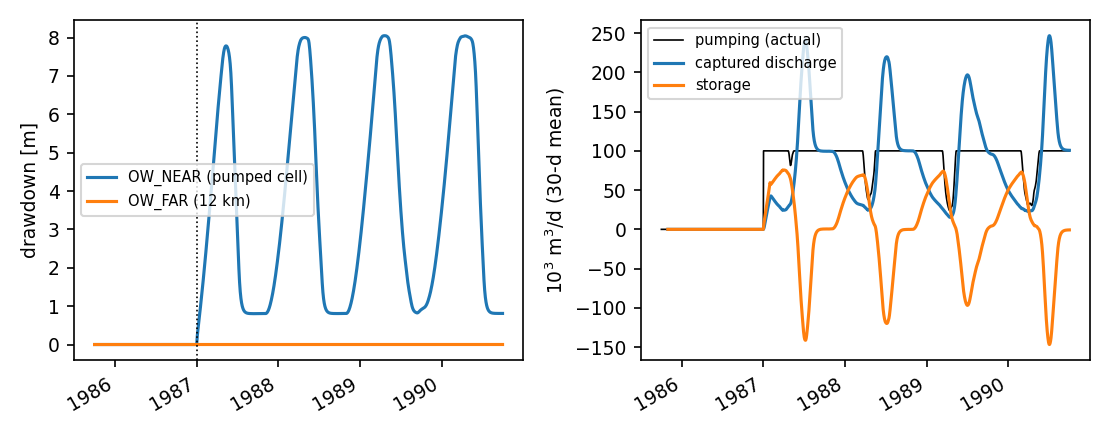
\includegraphics[width=\linewidth]{figures/fig_pumping.png}
\caption{Pumping test: drawdown at the monitoring wells (left) and where the pumped water comes from (right).}\label{fig:pumping}\end{figure}
\begin{figure}[!htbp]\centering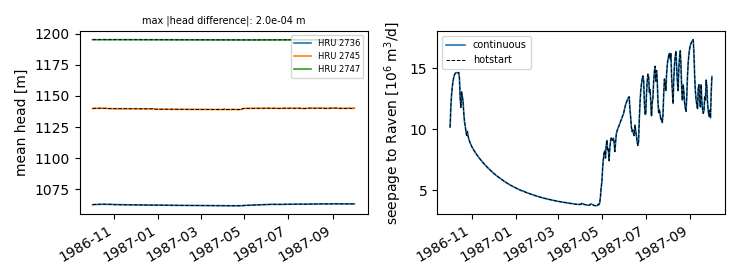
\includegraphics[width=\linewidth]{figures/fig_hotstart.png}
\caption{Restart: the second year of a continuous run (solid) and of a run restarted from \cmd{solution.rvc} (dashed).}\label{fig:hotstart}\end{figure}
\begin{figure}[!htbp]\centering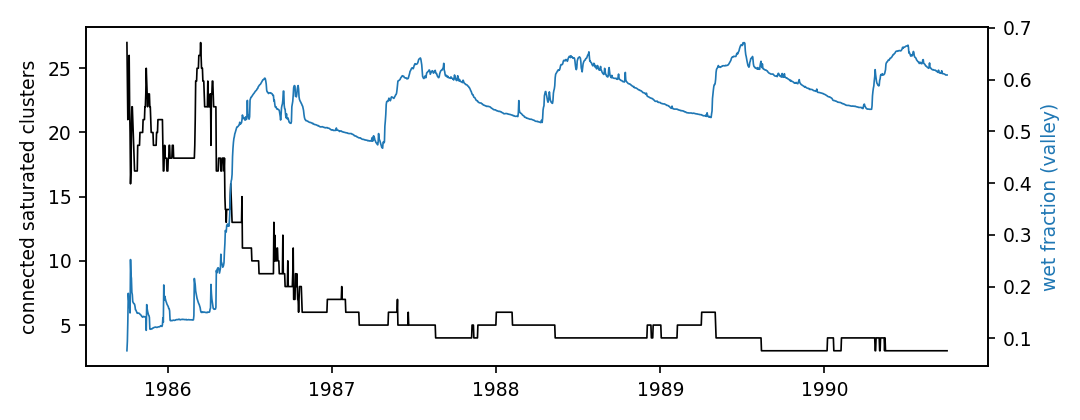
\includegraphics[width=0.9\linewidth]{figures/fig_connectivity.png}
\caption{Drying and rewetting: number of separate wet areas in the top layer (black) and wet fraction of the valley aquifer (blue).}\label{fig:conn}\end{figure}

\paragraph{Reservoirs that run dry.} In a 20-year test with a reservoir deliberately drawn empty by a minimum flow, the
reservoir's balance error is 13.7 million m$^3$: 1\,072 of its 1\,086 dry days balance exactly. Almost all of the rest
falls on the day after the reservoir empties, when the outflow still averages in the release rate at the end of the
previous day although the lake is empty. This lies in Raven's own reservoir routine, not in the coupling
(Section~\ref{ch:limits}, known issues).

\paragraph{River losses.} \cmd{tests/watershed\_balance.py} WB7--WB14 run a losing river (bed conductivity 20~m/d, the
water table 6~m deep, 40~mm/d of rain on days 1--3). A reach fed by an inflow hydrograph loses water from the inflow on
every step, and Raven's balance error stays at round-off ($3\times10^{-14}$~mm), also in a run restarted on a take day
and in each member of a 2-member ensemble. A headwater reach with a 10-day in-catchment unit hydrograph supplies its loss
from its outflow on the dry days: of 302.1~m$^3$ of leakage, 1.15~m$^3$ is still carried at the end (lost on the day the
reach stops flowing), and its outflow is 300.9~m$^3$ lower than without the river, the loss applied. With
\cmd{ROUTE\_DUMP} the reach stops flowing on day~4 and that day's 112.3~m$^3$ is carried, warned about and reported as a
run total. WB10 repeats the losing reach with every channel routing method (Muskingum and Muskingum-Cunge over 300~km,
storage coefficient, \cmd{ROUTE\_HYDROLOGIC}, diffusive wave and plug flow over 30~km), fed by an inflow that stops after
5 days: the volume leaving the watershed is lower than without the river by the loss taken (6\,539.9 against
6\,539.8~m$^3$ for Muskingum, within the file's digits) and the channel storage ends the same (the test allows
$10^{-5}$ of the loss taken, 0.065~m$^3$ for Muskingum; the run ends 0.007~m$^3$ apart), also with an irrigation demand on
the reach. WB11: a \cmd{ROUTE\_EXTERNAL} reach whose outflow a live file sets to
0.02~m$^3$/s every step delivers that outflow less the step's take (220.4~m$^3$/d), and its channel storage ends as without
the river. WB12: 2-member ensembles with \cmd{ROUTE\_HYDROLOGIC}, \cmd{ROUTE\_STORAGECOEFF} and \cmd{ROUTE\_TVD}, with and
without groundwater: every member's \cmd{Hydrographs.csv} (and \cmd{GWBudget.csv}) equals the single run's (the test
allows no difference without groundwater and $10^{-12}$ relative with it; the runs differ by 0). That member 1's
\cmd{Hydrographs.csv} and \cmd{WatershedStorage.csv} without groundwater are byte-identical to base Raven's member 1
was checked separately with base Raven for the three methods; WB12 does not run base Raven. WB13: the WB10 reach restarted with another \cmd{:TimeStep}
(0.5 then 1~d, 1 then 0.25~d) right after a take from the outflow or from the inflow, with \cmd{ROUTE\_HYDROLOGIC} and
\cmd{ROUTE\_STORAGECOEFF}: the outflow leaving the watershed over both parts is lower than without the river by the leakage
MODFLOW received (2\,980.96 against 2\,981.16~m$^3$, the file's digits), the channel storage ends the same (the test
allows $10^{-5}$ of the leakage, about 0.03~m$^3$; the runs end within $10^{-11}$~m$^3$) and Raven's balance error stays
at round-off.
WB14: the same reach with \cmd{ROUTE\_DIFFUSIVE\_WAVE}, whose inflow history Raven averages to a longer step, restarted
right after a take from the inflow, in five chains of \cmd{:TimeStep}: 0.5 then 1~d; 0.25 then 1~d; 0.25, 0.5 for half a
day, then 1~d; and two with a middle part of one step, 0.1, 0.2, 1~d and 1, 0.2, 1~d. In every part Raven's balance error
of the river run equals that of the same run without the river (the test allows $10^{-6}$~mm; the runs differ by at most
$6\times10^{-14}$~mm; the runs without the river carry Raven's own error of up to 2.2~mm in the chains with a one-step
part, Section~\ref{ch:limits}), and the leakage equals the lower outflow plus the lower channel storage at the end (the
test allows 0.5~m$^3$ plus $10^{-5}$ of the leakage; 2\,910.19 against 2\,910.11~m$^3$ for 0.5 then 1~d, the file's
digits). A restart (0.5 then 1~d) from a \cmd{solution.rvc} without \cmd{:GWRiverInflowTakes}, written by
\cmd{RAVEN\_EXE\_REF}, has no larger balance error than that build's own restart from the file (0.01742~mm in both; run
only when \cmd{RAVEN\_EXE\_REF} is set). WB14's reach is fed by a steady inflow; with takes on a reach upstream, the
restart books the takes exactly, and Raven's averaging of the downstream inflow history adds its own error (Section~\ref{ch:limits}).
\cmd{tests/boundary\_recharge.py}: an HRU over specified-head cells whose polygon reaches 0.05~m into a
neighbouring cell gives that 10~m$^2$ sliver its own share of the recharge only (399.9 of the 400~m$^3$/d go to the
specified heads; seepage to Raven 135.1 against 134.8~m$^3$/d without the sliver). The same holds for an HRU without soil under \cmd{:SoilZone PHYSICAL} (BR3: 799.8 of 800~m$^3$/d to the specified heads).

\section{Independent checks}\label{sec:independent}
\subsection{Geometry against standard libraries}
The geometry functions are compiled into a stand-alone test and compared with widely used libraries
(Table~\ref{tab:geom}); the readers of the spatial inputs are checked against the same libraries and against files
that must be refused (Table~\ref{tab:readers}).
\begin{table}[!htbp]\centering
\caption{Geometry functions against independent libraries.}\label{tab:geom}
\begin{tabularx}{\linewidth}{Y P{0.22\linewidth}P{0.2\linewidth}}\toprule\hdr
Function & Reference & Largest difference\\\midrule
Polygon clipping and area (400 random, mostly concave polygons) & shapely & $4.6\times10^{-12}$ (relative)\\
Equal-area projection (300 points over the Liard region) & pyproj (same sphere) & $6.7\times10^{-7}$ m\\
Albers and Lambert conformal conic projections (ten cases, also with the origin at either pole and with false eastings) & pyproj (PROJ) & $4.7\times10^{-7}$ m\\
Projection round trip & -- & exact\\
Bilinear raster sampling of a plane, which bilinear sampling reproduces exactly (200 points); the no-data margin of half a cell beyond the edge & the plane & $3.6\times10^{-15}$; a value 0.4 cell beyond the edge, none 0.6 cell beyond\\
\cmd{:InputCRS}: a UTM raster holding a plane, sampled at 300 lon/lat points & pyproj (PROJ) & $3\times10^{-10}$ (of values $\sim10^3$)\\
\cmd{:InputCRS}: UTM GeoJSON polygons and lines read back in lon/lat & pyproj (PROJ) & $1.1\times10^{-11}$ degrees\\\bottomrule
\end{tabularx}
\end{table}
\begin{table}[!htbp]\centering
\caption{Readers of the spatial inputs against independent libraries and reference files.}\label{tab:readers}
\begin{tabularx}{\linewidth}{Y P{0.22\linewidth}P{0.2\linewidth}}\toprule\hdr
Input & Reference & Result\\\midrule
GeoJSON and ASCII-grid variants (3-D coordinates, string IDs, holes, cell-centre headers, \dots) & shapely, reference values & read correctly\\
GeoJSON numbers (14 files): coordinates that are strings, \cmd{null}, \cmd{true} or too large; \cmd{NaN}, \cmd{Infinity}, hexadecimal numbers and leading zeros; features with and without \cmd{"properties"} & the JSON standard & the invalid ones refused, naming the feature, ring and vertex or the line and column; a feature without \cmd{"properties"} refused only where an ID is read\\
\cmd{:InputCRS}: projected \cmd{"crs"} member without \cmd{:InputCRS}, another projection, lon/lat file with \cmd{:InputCRS}, projected coordinates or raster without \cmd{:InputCRS} & -- & refused\\
\cmd{"crs"} members: EPSG:4326, 4269, 4617, 6318, 4979, 4267, a versioned URN (\cmd{EPSG:6.6:4326}), an \cmd{opengis.net} URL (4269), OGC CRS83; a versioned URN of UTM 10N; EPSG:3157 and 4647 (projections, not built in) & EPSG registry (pyproj) & geographic ones read as lon/lat (refused with \cmd{:InputCRS}); the URN read by its code; 3157 and 4647 ask for their parameters, which are then accepted\\
\cmd{"crs"} EPSG:2227 (US survey feet); a file with a UTF-8 byte-order mark; \cmd{:InputCRS} with letters or units in a parameter (\cmd{-ll7}, \cmd{O.9996}, \cmd{500km}), surplus or missing values, an unknown ellipsoid, \cmd{EPSG:32610x} & -- & 2227 refused; the file read; each specification refused, naming the parameter or value (\cmd{geomtest\_check.py})\\
GeoTIFF reader: 228 files written by GDAL and tifffile (every compression, predictor, sample type and byte order; strips and tiles, classic and BigTIFF; NODATA; internal masks; PixelIsPoint; EPSG codes; GDAL's band scale and offset, and role-less items of those names) & their ESRI ASCII twins & every value and the corner exact; the same samples bit for bit\\
ESRI ASCII grids: GDAL's \cmd{dx}/\cmd{dy} header (with corner or centre), \cmd{NODATA\_value nan}; more values than \cmd{ncols}$\times$\cmd{nrows}, a wrapped grid, fewer values, an unknown key, a value or header value that is not a number & the GeoTIFF with the same pixels; the $-9999$ twin & the same samples bit for bit; each malformed grid refused with its reason\\
GeoTIFF reader: 34 unsupported or damaged files (also a prime meridian given only by its longitude or by the datum, a projected code in feet without its units key, a band unit in feet), an oversized file, and damaged copies of every fixture (bytes changed, cut, inserted, random) & -- & each refused with its reason; no crash (also under AddressSanitizer)\\\bottomrule
\end{tabularx}
\end{table}

\paragraph{GeoTIFF rasters.} \cmd{tests/geotiff/geotiff\_check.py} reads 228 GeoTIFF files written by GDAL and tifffile
(every supported compression, predictor, sample type and byte order, in strips and tiles, classic and BigTIFF, with
NODATA values, internal masks, \cmd{PixelIsPoint} and several EPSG codes) and compares each with an ESRI ASCII twin holding the same
values: the corner, cell size and every value agree exactly, and Raven's sampling of the two at 4\,000 points agrees bit for
bit; rasters with rectangular pixels agree with an independent bilinear sampler. Each of 186 of these files used as \cmd{:LandSurface} of a small model, and 43 as \cmd{:BedrockSurface}, gives outputs
byte-identical to its twin (the model files hold the sampled cell elevations); so do projected rasters under
\cmd{:InputCRS}. Unsupported, damaged and oversized files, a code that disagrees with \cmd{:InputCRS}, and a DEM or bedrock
raster that covers no active column stop the run with their reason; a raster covering part of the columns gives a warning
with their number. Damaged copies of every file (bytes changed, cut or inserted, random content) are refused with a message
or read, never crash the reader (also checked once under AddressSanitizer and UndefinedBehaviorSanitizer).

\paragraph{Projected input files.} The Liard example with every geometry and raster input converted to UTM zone 10
(\cmd{tests/crs\_inputs.py}, PROJ through pyproj, \cmd{:InputCRS EPSG:32610}) gives the same grid as the example in
longitude/latitude: the same active columns and cells, river, boundary and well cells, polygon areas within
$8\times10^{-12}$ and HRU--cell overlaps within $1.1\times10^{-9}$ of a cell; without rasters the hydrographs agree to the
printed digits and the groundwater budget within $2\times10^{-8}$ over 120 days. With the DEM and bedrock resampled to
300~m UTM grids the model top differs by 0.018~m on average (the resampling) and the hydrographs by $10^{-3}$. Projected
files without \cmd{:InputCRS}, files in another projection and wells given by \cmd{X} and \cmd{Y} without \cmd{:InputCRS}
stop the run with a message naming \cmd{:InputCRS}; with \cmd{:InputCRS}, a DEM, a bedrock raster, the HRU polygons or a
boundary line left in longitude/latitude stop the run as ``looks like longitude/latitude''. The boundaries of this test have
heads above their cells (the general-head line by its \cmd{HEAD}, the specified-head lake by a \cmd{:BoundaryHead} series
with \cmd{HEAD 0}), and both runs give them the same cells (3 and 9).

\paragraph{A layer that starts dry.} The start-up warning for a layer that starts dry (\cmd{tests/dry\_start.py}) names
layer~2 of the Liard model with \cmd{INITIAL\_HEAD\_DEPTH} 25~m (2\,794 cells), and is absent with a steady-state start
and for the example as shipped, whose outputs equal those of the reference build.

\paragraph{Budget file and particle tracking.} With \cmd{:WriteGWBudgetFile} (\cmd{tests/budget\_file.py}, the Liard
example with a pumping well) MODFLOW's budget file holds \cmd{FLOW-JA-FACE}, the specific discharge, the saturation and
every package at every step, and its package totals equal \cmd{GWBudget.csv} within $4\times10^{-10}$; \cmd{gwf.porosity}
holds each cell's class porosity. The solution is the same with and without the option, and without it the \cmd{mf6}
folder equals the reference build's. \cmd{tools/make\_prt.py} runs MODFLOW~6 PRT on these files through the library:
eight particles around the well, tracked forward and backward, move in opposite directions; with a steady-state first
period each is released once, at the start (forward) or end (backward) of Raven's run, and ends within it. With flows
saved every fifth step only (\cmd{:HeadSaveFrequency 5}) the script stops, in both directions, with a message naming
\cmd{:HeadSaveFrequency 1}.

\subsection{Exchanged flows against MODFLOW's own budget}
MODFLOW writes its own volume budget in its list file. For runs covering every package, every flow the coupling exchanged
is compared with MODFLOW's figure for the same step, read by package name (\cmd{tests/budget\_xcheck.py};
Table~\ref{tab:listcheck}); the differences are at the printing precision of the list file. The check fails when it
compares nothing.
\begin{table}[!htbp]\centering
\caption{Coupler flows against MODFLOW's list-file budget.}\label{tab:listcheck}
\begin{tabularx}{\linewidth}{P{0.25\linewidth}Y P{0.2\linewidth}}\toprule\hdr
Run & Packages compared & Largest difference\\\midrule
20-year Liard & recharge, drains, rivers, storage & $6.2\times10^{-7}$\\
Pumping and boundaries & + wells, general-head boundaries & $6.9\times10^{-7}$\\
Fixed head and delay & + fixed heads & $6.1\times10^{-8}$\\
Wetland exchange & + store exchange & $1.1\times10^{-7}$\\
Reservoir & + reservoir seepage & $2.6\times10^{-7}$\\
Drying & + water-table ET & $4.1\times10^{-8}$\\\bottomrule
\end{tabularx}
\end{table}

\subsection{Grid size and time step}
The accounts stay exact for any cell size and time step (Table~\ref{tab:invariance}; subbasin 52, one year). The first
rows use a head tolerance of 0.01~m; with it the worst single step on 4~km cells is 0.47\% of the flow, and the default
tolerance of 0.00001~m brings it down to 0.002\%. Raven's balance stays at its first step's value on every step (base
Raven's for this model: 0.431~mm with daily steps, 0.216~mm with half-day steps).
\begin{table}[!htbp]\centering
\caption{Invariance to cell size and time step.}\label{tab:invariance}
\begin{tabular}{lrlrr}\toprule\hdr
Set-up & Active columns & Recharge & Worst step & Raven balance\\\midrule
1 km cells & 2\,147 & exact & 0.029\% & 0.431 mm\\
2 km cells & 545 & exact & 0.092\% & 0.431 mm\\
4 km cells & 142 & exact & 0.47\% & 0.431 mm\\
4 km cells, default tolerance & 142 & exact & 0.002\% & 0.431 mm\\
2 km cells, half-day steps & 545 & exact & 0.059\% & 0.216 mm\\\bottomrule
\end{tabular}
\end{table}

\section{Model files and faulty input}\label{sec:mf6files}
Raven writes every MODFLOW input file, and \cmd{grid\_cells.geojson}, before it loads the MODFLOW library; in the
existing-model mode it also copies the model and prepares the simulation, time and name files first. Almost everything
except the solve itself can therefore be checked without MODFLOW, by pointing \cmd{RAVEN\_MF6\_LIB} at a file that does not
exist: the run then stops, with a message, just after the files are written. The checks of this section use this, and
run again with the library where it matters.

\paragraph{MODFLOW input files.} \cmd{tests/mf6files\_check.py} builds 16 set-ups over every grid type, rotation,
refinement, layers by elevation, aquicludes, boundaries, wells, lakes and imported cells, and checks the files Raven
writes: FloPy reads every model; cells are valid and do not overlap; the grid origin and rotation agree with the cell file
(0.5~m); DISV and DISU vertices are right; DISU connections are symmetric; face angles agree with the vertices
(1\textdegree); no vertical connection passes through an aquiclude; drains lie inside the top cell; boundary polygons
select the right cells. All 127 checks pass.

\paragraph{Faulty and unusual input.} Thirty-nine faulty or unusual set-ups of the Liard model check the messages
(Table~\ref{tab:faulty}): every error stops the run with a message that names the problem --- no crash --- and every
tolerated case runs. \cmd{tests/edge.py} adds 36 generated-model and 17 existing-model set-ups, judged without and with
MODFLOW; the valid existing-model preparations are checked in detail (stress periods split at the start date, restart
renumbering, the original model untouched). All 53 behave as required.
\begin{table}[!htbp]\centering
\caption{Response to faulty or unusual input.}\label{tab:faulty}
\begin{tabularx}{\linewidth}{Y P{0.4\linewidth}}\toprule\hdr
Input & Response\\\midrule
Missing HRU file or ID field; unknown profile or class; malformed class row & stops; names the file, field, profile or row\\
Aquiclude as top layer; zero layer thickness; value out of range ($K\le0$, $S_y>1$, negative delay, \dots) & stops; names the parameter\\
Process draining \cmd{GROUNDWATER} in a coupled HRU; no process feeding it & stops; names the process and HRU\\
Wrong library path; missing raster; well outside the model & stops; names the path, file or well\\
DEM or bedrock raster that covers no active column (another area, a wrong corner, NODATA only) / covers part of them & stops with both extents / warns with the count\\
Duplicate IDs or names; two exchanges on one store; boundary without \cmd{HEAD} & stops; names the item\\
Malformed groundwater command in \cmd{.rvg}, \cmd{.rvt} or \cmd{.rvc} & stops; names the command\\
Hotstart heads for a different grid; cells larger than the HRUs & stops; explains the mismatch\\
Monitoring well outside the model; unknown \cmd{.rvg} command & runs with a warning\\
\cmd{TO\_BEDROCK} in a middle layer; no DEM or bedrock map; coupling switched off & runs as documented\\
Malformed numbers in the \cmd{.rvg} (\cmd{:GridCellSize 2,000.0}, \cmd{2km}, \cmd{HEAD H1146}, \cmd{1146.85m}, \cmd{50.5} iterations, a \cmd{:Wells} value); a cell size giving more than $5\times10^6$ cells per layer (\cmd{:GridCellSize 50} and \cmd{60} on Liard), a refinement size giving more on a regular grid (counted with its 2:1 smoothing: 60 short lines on 400~$\times$~300~km, N24) or, by its estimate, on a quadtree grid (\cmd{:GridRefinement RIVERS 0.1}) & stops before the grid is built; names the command and the value or the estimated cells per layer (\cmd{tests/input\_checks.py})\\
A quadtree grid within the limit that needs more memory than there is (\cmd{RIVERS 0.5} on Liard, about $4.6\times10^6$ cells per layer, under a 3~GB limit) & stops naming \cmd{:GridRefinement} and the estimated cells per layer (no crash)\\
Overlapping and adjacent refinement features: 200 copies of one line (\cmd{LINES 0.1}) and 20 adjacent squares (\cmd{POLYGONS 0.5}) on a 4-HRU strip & built (the estimate counts each square once)\\
An HRU mesh of 4 HRUs of 5~$\times$~5~km with 500~m cells and one short refinement line of 0.1~m (N17) and of 2~m (N18) & N17 stops before the mesh is built (``too slow to build''); N18 is built within 120~s (65\,484 cells per layer)\\
Boundary polygons that overlap: two features, the same feature twice, a MultiPolygon of two overlapping parts (N19) & each selects the cells of the union (as the larger polygon alone)\\
Malformed numbers in the \cmd{.rvp} aquifer tables: \cmd{K\_HORIZ 1O}, \cmd{SPEC\_YIELD O.2}, a thickness \cmd{3m}, a profile parameter \cmd{2.O} (N20--N23) & stops; names the table, the row and the token\\
Malformed numbers in the \cmd{.rvc}: \cmd{:InitialGWHeads ELEVATION 98,5}, \cmd{H98.5} or \cmd{0x62}, \cmd{:InitialGWHeads FROM\_PROFILE 0}, a \cmd{:GWHeads} value \cmd{98.5x} & stops; names the command and the token (\cmd{test\_inputs.py} I22)\\
\cmd{:WellFlowRate} in \cmd{m3/s} or \cmd{L/s}; other units of a well or head series & converted to m$^3$/d (5\,000 m$^3$/d either way); stops\\
A package of an existing model named like one of Raven's (\cmd{DRN\_RAVEN}); a recharge package so named and taken over & stops with Raven's message; runs\\\bottomrule
\end{tabularx}
\end{table}

\section{Randomized testing}\label{sec:fuzz}
A test driver (\cmd{tests/fuzz\_grids.py}) builds random but valid set-ups of the subbasin-52 model, drawing every option
at random: grid type (regular, rotated and refined, quadtree, HRU mesh, imported cells, layers by elevation), rotation,
refinement and XT3D, cell size (1--3 km), minimum coverage, one-day or half-day steps, conductivities, initial depth,
seepage leakance and smoothing, water-table ET, recharge delay, steady-state start, wetland exchange, 0--2 pumping wells,
monitoring wells, a general-head boundary, a fixed-head area and a coupled reservoir. Every run is checked independently of
the audit tool: exact recharge, seepage, river, store and reservoir identities; MODFLOW's balance (every converged step
below 0.1\%, cumulative below $10^{-4}$); Raven's balance below 1 mm; agreement with MODFLOW's list file; and, for about a
third of the set-ups, a restart that must reproduce the continuous run (every flow within $10^{-4}$ of its largest value in
the run).

With MODFLOW 6.8.1, three batches of 24 (72 set-ups: 10 regular, 11 rotated and refined, 16 quadtree, 15 HRU mesh,
6 imported, 14 with layers connected by elevation; 49 with a reservoir; 20 with a restart comparison, largest deviation
$3.1\times10^{-6}$) and two batches of 12 that always have a reservoir and lake refinement (24 set-ups, 6 with a restart) all
pass every check, including MODFLOW's list-file budget and the reservoir identity. The optional fully implicit XT3D can
fail to converge where cells dry and rewet (in one random set-up on 38 of 45 days, with exact accounts on the converged
days and the safeguard limiting the exchange on the others); it is therefore off by default.

\section{Grid types}\label{sec:vgrids}
\begin{plain}
Every kind of grid is checked in four ways: its cells cover the area exactly with no gaps or overlaps; two different ways of
handing the same cells to MODFLOW give the same answer; the answer matches an exact textbook solution and gets closer to it
as the cells get smaller; and a restarted run matches a continuous one.
\end{plain}
Every grid option is verified the same way as the default grid, plus the checks below.

\paragraph{Geometry of the grids.} A stand-alone test (\cmd{tests/gridtest.cpp}) checks every generator: cells tile the
domain exactly (area sums equal to $10^{-15}$), neighbours are symmetric, each cell's perimeter equals its shared faces plus
the domain edge, Voronoi connections are exactly orthogonal, quadtree neighbours differ by one level at most, clipping
handles concave cells and lattices of cocircular seeds, and grids survive the linkage cache bit for bit. It also checks
that the grid-size stop names its cause (the cell size, a refinement, the seeds of an HRU mesh, an imported grid or an
existing model).

\paragraph{Two formats, one answer.} The quadtree cells were run once as DISV (MODFLOW computes the geometry) and once
imported as DISU (the coupler computes connection lengths, face widths and directions): all flows agree to $6\times10^{-7}$ and
water tables to 0.3 mm. A regular grid written as DISU gives heads identical to DIS. Solving the coupler's DISU equations
independently in Python reproduces MODFLOW's heads to $3\times10^{-8}$ m.

\paragraph{Analytical solution.} A textbook case has an exact answer to compare with: a single well pumping from an aquifer
whose water level is held fixed all around, far away (the \emph{Thiem} solution). Close to the well the water level falls in
a known way with distance. A well pumping 5\,000 m$^3$/d from a confined aquifer ($T=500$ m$^2$/d) inside a
20 km square with fixed heads on its edge should give the Thiem profile $h=A+\frac{Q}{2\pi T}\ln r$. The slope fitted to
all cells between four cell sizes and 3 km from the well is compared with $Q/(2\pi T)$ in Table~\ref{tab:thiem}: every grid
converges to the analytical value as its cells shrink, and the solutions are symmetric around the well (slopes in the four
directions within 0.6\%).

\begin{table}[!htbp]\centering
\caption{Thiem test: error of the fitted slope $\partial h/\partial\ln r$ (\cmd{tests/thiem}, MODFLOW 6.8.1; every run
checked, none with a failed step).}\label{tab:thiem}
\begin{tabular}{lrrr}\toprule\hdr
Grid & Coarse & Medium & Fine\\\midrule
Regular, 500 / 250 / 125 m & +0.60\% & +0.04\% & +0.01\%\\
Regular 250 m, rotated 17\textdegree & & +0.03\% & \\
Regular 1 km refined to 125 m at the wells & & +1.01\% & \\
Quadtree, base 1\,000 / 500 / 250 m, 62.5 m at the wells & +0.80\% & +0.59\% & +0.26\%\\
Imported cells (the 250 m quadtree) & & & +0.25\%\\
HRU mesh, 500 / 250 m (250 m with XT3D) & +0.57\% & +0.29\% & $-$0.06\%\\\bottomrule
\end{tabular}
\end{table}

\paragraph{Lakes.} A reservoir with seepage to the aquifer was placed on the largest coupled HRU of subbasin~52 and each
refinable grid (3~km cells) was refined around it with \cmd{LAKES} (\cmd{tests/lake\_test.py}). The median size of the
cells touching the lake falls from 3\,000 to 750~m (rotated regular grid), from 3\,000 to 375~m (quadtree) and from 1\,210 to
490~m (HRU mesh); a \cmd{POLYGONS} file with the same outline gives the same mesh. The water accounts stay exact (MODFLOW
residual below $1.2\times10^{-11}$), and the reservoir's seepage reaches MODFLOW exactly one step after it leaves the lake
(sent $=$ previous step's volume in transit to $1.6\times10^{-10}$; delivered $=$ sent); MODFLOW's own list-file budget shows
the same reservoir seepage.

\paragraph{Restarts.} For every grid type a 60-day run is compared with a 30-day run restarted from its
\cmd{solution.rvc} (\cmd{tests/restart\_test.py}: subbasin-52 model with 3~km cells, a pumping well and half-day steps):
regular $9.9\times10^{-7}$, rotated and refined $1.9\times10^{-7}$, quadtree $4.4\times10^{-7}$, HRU mesh $1.9\times10^{-7}$,
layers by elevation $8.3\times10^{-8}$, with exact water accounting in all.

\paragraph{Randomized testing.} The randomized set-ups of Section~\ref{sec:fuzz} draw the grid type at random; their
restart criterion scales each day's difference by the flow's largest value in the run, as the existing-model tests do.

\section{Coupling an existing model}\label{sec:vexisting}
\begin{plain}
The existing-model mode is tested on a MODFLOW model built independently of Raven. It is also tested on a copy of that
model in feet and seconds, which must give the same answers; on a model that Raven built itself and then read back in, which
must reproduce Raven's own run; with restarts; with deliberately wrong input, which must be caught; with random set-ups;
and with two models of the USGS example collection. In every run no water is created or lost.
\end{plain}
The existing-model mode is tested on the synthetic Liard model of Chapter~\ref{ch:existing} (a rotated UTM grid, four
layers, monthly stress periods, wells, rivers and a head boundary), built independently of Raven
(\cmd{tests/existing/make\_ext\_model.py}), and on a feet/seconds copy of it. Every run keeps the water accounts exact:
Raven's recharge reaches MODFLOW exactly, the MODFLOW residual including the model's own packages is about
$2\times10^{-11}$, seepage and river exchange balance to $10^{-11}$, and no step fails.

\begin{table}[!htbp]\centering
\caption{Existing-model mode: tests and results.}\label{tab:vexisting}
\begin{tabularx}{\linewidth}{P{0.42\linewidth}Y}\toprule\hdr
Test & Result\\\midrule
Built-in projections against PROJ (9 systems, 18\,000 points) & largest difference 3 micrometres\\
Cell outlines from MODFLOW (\cmd{:MF6CRS}) against a cell file & recharge identical; other flows within $3.5\times10^{-7}$\\
Feet and seconds against metres and days & recharge identical; other flows within $4.6\times10^{-6}$\\
Round trip: a Raven-generated model re-imported & recharge identical; outlet flow within $1.7\times10^{-6}$\\
\cmd{:OverlapWeights} (computed in UTM) against cell outlines & recharge identical; seepage within $4.5\times10^{-7}$, rivers within $4\times10^{-6}$\\
Restarts (inside a stress period; before a change of well rates) & within $1.4\times10^{-7}$; the renumbered well data switch on the right date\\
Water-table ET, surface-store and reservoir exchange (\cmd{EVT\_RAVEN}, \cmd{SWX\_RAVEN}, \cmd{RES\_RAVEN}), metres/days and feet/seconds, 120 days (\cmd{tests/existing/ext\_exchanges.py}) & accounts exact (MODFLOW residual below $4\times10^{-11}$); each package's flows in MODFLOW's budget file and list file equal \cmd{GWBudget.csv} (within $4\times10^{-10}$; the list file to its printed digits); water-table ET at most 5\% of the unmet PET on any day; feet/seconds: the exchanged flows within $10^{-7}$, the other columns within $2\times10^{-5}$ (one step of 120 days; the two models are solved separately to the same tolerance); a restart with reservoir seepage in transit within $3\times10^{-7}$; a kept EVT package with \cmd{EXTINCTION\_DEPTH} refused\\
Later starts (\cmd{ext\_inputs.py}, \cmd{restart\_ext.py}): TDIS and water-mover rows in \cmd{OPEN/CLOSE} files; wells driven by a TS6 series, restarted between two of its entries; 6-hour steps restarted at 12:00; DIS6 and STO6 under names of their own in the name file & identical to the runs with the rows inline; within $4.2\times10^{-7}$ and $2.3\times10^{-6}$ of the continuous runs; \cmd{TAS6} refused; the renamed packages read (\cmd{GWBudget.csv} identical to the usual names', MODFLOW's storage flows kept)\\
Dry and specified-head cells under the exchanges (\cmd{ext\_exchanges.py}): water-table ET in a model without \cmd{NEWTON} whose top cells dry (MODFLOW moves the ET to the cell below); a reservoir over cells that become specified heads (all, or 2 of 5); a reservoir over dry cells without \cmd{NEWTON} & water-table ET equal to MODFLOW's budget file on every saved step, MODFLOW error $5\times10^{-3}$~m$^3$/d on $6\times10^{5}$~m$^3$/d; the reservoir books exact (sent = delivered $-$ gain not supplied $+$ not delivered), seepage not delivered $6.4\times10^{5}$~m$^3$ returned and its run total equal to its column, all of it delivered when 3 of 5 cells remain; no HDRY or NaN in the outputs\\
Safeguards (14 faulty set-ups, \cmd{guards.py}) & every one stops with a message naming the problem\\
Randomized set-ups (units, link, stream mapping, seepage, ET kept or taken over, coverage, restarts; \cmd{fuzz\_ext.py}); checked with the audit identities and MODFLOW's own budget file & 20 of 20 pass, 6 with a restart (within $2.7\times10^{-7}$); MODFLOW's saved flows of Raven's packages agree to $10^{-10}$\\
Sanitizers (AddressSanitizer, UndefinedBehaviorSanitizer) on the coupling's code: both units, all three links, seepage off, restarts & no error\\\bottomrule
\end{tabularx}
\end{table}
The test model allows 300 outer iterations. Its metres/days version needs 288 of them in its first (steady-state)
period, and the feet/seconds version a few more, so one feet/seconds set-up does not converge on that step while its twin
does; every later step takes the same number of iterations in both, and with 500 iterations both converge on every step.
The weights test shows why the overlaps are normalised per HRU: the weights were computed in the model's projection, whose
areas differ from Raven's by about 0.5\% at this latitude, and the recharge volumes still agree exactly. In the two-year
example the stream package loses about 3.8 million m$^3$/d to the aquifer; the small headwater reaches cannot always supply
their share, so up to 106 million m$^3$ of river loss is carried from step to step at times --- all of it supplied by the end
of the run, as the accounting requires.

\subsection{USGS example models}\label{sec:usgs}
Two models of the USGS MODFLOW~6 example collection (\cmd{mf6examples.zip}) are coupled as existing models with
\cmd{:OverlapWeights}. They are not georeferenced, so the Liard HRUs of subbasin~52 are laid over each model's active cells,
with \cmd{.rvh} areas equal to their zones so that Raven's recharge depths become the same depths on the model
(\cmd{tests/existing/usgs\_sagehen.py}, \cmd{usgs\_capture.py}).

\paragraph{Sagehen Creek} (a real watershed in the Sierra Nevada: 73$\times$81 cells of 90~m, one convertible layer,
Newton, a steady-state day and 398 daily periods, an unsaturated-zone package (UZF) whose rejected infiltration and
groundwater discharge the water mover (MVR) sends to streams (SFR), land-surface drains also moved to SFR, three specified
heads). Raven takes over the UZF package, so its recharge replaces the model's infiltration, and removes the 3\,375 movers
that name it from the working copy. The recharge identity, the river bookkeeping and the seepage returned are exact in every
case; the water the model's packages pass to the mover is part of MODFLOW's balance. MODFLOW's cumulative residual is
$8.5\times10^{-7}$ with the model's own loose solver (\cmd{OUTER\_DVCLOSE} 0.03~m, \cmd{INNER\_RCLOSE} 1\,000~m$^3$/d),
$2.8\times10^{-10}$ with a tight solver, and $1.3\times10^{-11}$ with Raven's seepage drains beside the model's own. A
restart at day~200, inside the daily periods (the mover renumbered), reproduces the continuous run to $3.3\times10^{-8}$.
Keeping the UZF package beside Raven's recharge (recharge counted twice, the user's choice) runs with exact accounts; one
day of the snowmelt peak misses the tight tolerance and is flagged. The drains as Raven's stream package are refused,
because the mover already sends their water to SFR.

\paragraph{Stream capture} (a steady-state model: 40$\times$20 cells of 250~m, time in seconds, one stress period of one
second, a river, six pumping wells, specified heads). Raven recognises the steady-state model and stretches its period over
the 60-day run, so each day is a steady-state solution; the storage column stays zero. The river carries its exchange to
Raven's reaches (subbasin of the dominant HRU); recharge identity and river bookkeeping are exact, MODFLOW's residual is
$2.8\times10^{-9}$, and a restart at day~30 reproduces the continuous run to $1.0\times10^{-7}$. With the model's own
tolerance of $10^{-8}$~m and 100 outer iterations, four days do not converge; they are flagged and the accounts on the
other days are exact. The Liard seepage leakance of 1/d lets the water table of this thin, flat-topped aquifer reach the land
surface on the wettest days, where MODFLOW's Newton solver does not converge on two of them; 0.01/d, suited to its
conductivity of about $7\times10^{-5}$~m/s, converges every day.

\subsection{MODFLOW versions}\label{sec:mf6versions}
Every test of \cmd{tests/run\_all.py} has been run with MODFLOW~6.8.1 and~6.6.3. Raven writes the \cmd{NEWTON} option
without its \cmd{UNDER\_RELAXATION} keyword (Section~\ref{ch:mf6}): with that keyword MODFLOW~6.6.3 resets a head that falls
below the cell bottom, the Newton change of a drying thin aquitard cell repeats unchanged at every iteration, and the default
Liard grid fails to converge on 295 of 344 days. Without it, every step passes with both versions with the same numbers: the
Liard grid table agrees to the last digit shown. For existing models Raven reads the library's version and warns when a model
uses the keyword with a version before~6.8.

% Verification of the soil zone (tests/soilzone): test models, the column and the hillslope, the water table in every
% position, the interface and MODFLOW's side, the unsaturated-zone methods, inputs and robustness.
\section{The soil zone}\label{sec:vsoilzone}
The soil-zone coupling (Section~\ref{ch:soilzone}) is tested at three levels: the unsaturated column and the capillary rise
relation on their own against independent solutions; small coupled models that put the water table in each of the
positions of Figure~\ref{fig:szregimes}; and the same models coupled again as existing MODFLOW models. The tests in
\cmd{tests/soilzone} build small synthetic models (\cmd{sz\_models.py}: a generated MODFLOW model under Raven HRUs with
soil, forcing written by the script) and compare them with exact values or with a MODFLOW-only reference in which the soil
zone is a MODFLOW layer and a drain at the land surface takes the overflow (\cmd{sz\_reference.py}); only LP1 starts from the
Liard example. Every coupled run is also checked by \cmd{sz\_check.py}, which closes, step by step, MODFLOW's balance,
Raven's balance and the recharge, soil-zone and unsaturated-zone identities of Section~\ref{sec:accsz} at their standard
limits (recharge $5\times10^{-9}$, soil zone and columns $10^{-8}$ relative, from the first step; \cmd{sz\_check.ID\_LIMITS}),
and requires no soil-zone shortfall. Its self-test shows that the column identity catches a small leak: exact books give 0,
and a leak of $10^{-4}$~m$^3$ per step on a 9\,776~m$^3$ store gives $2.4\times10^{-7}$ and fails. The numbers below are those
of the full mode of \cmd{tests/run\_all.py} with MODFLOW~6.8.1, except where a table says otherwise.

\subsection{The column, the hillslope and the interface}\label{sec:vszbasic}
\begin{longtable}{P{0.13\linewidth}P{0.42\linewidth}P{0.36\linewidth}}
\caption{The column, the hillslope, time steps, restarts and the Liard model (\cmd{soilzone\_unit}, \cmd{spike\_xmi},
\cmd{test\_column}, \cmd{test\_hillslope}, \cmd{test\_dynamics}, \cmd{test\_restart}, \cmd{test\_liard\_physical}).}\label{tab:vszbasic}\\
\toprule\hdr Test & What is checked & Result\\\midrule\endfirsthead
\caption[]{The column, the hillslope and the interface (continued).}\\
\toprule\hdr Test & What is checked & Result\\\midrule\endhead
Unit & \cmd{soilzone\_unit.cpp}: filling and draining of the layers, the sub-grid level and its inverse, the contact weights and flux derivatives against finite differences, continuity across the sample bases, the local solve (monotone, root, mass), the Robin slope; 20\,000 random cases each & 57 checks, 0 failed\\
XMI & \cmd{spike\_xmi.py}: values written between MODFLOW's outer iterations through XMI (GHB \cmd{BHEAD}/\cmd{COND}, RCH \cmd{RECHARGE}) reach the solver; the coefficients are recomputed every outer iteration; a solve after convergence is a normal iteration & all three hold (MODFLOW 6.8.1)\\
CT1 flat column & closed column, $S_y$ = drainable porosity = 0.2, recharge 10~mm/d: the water table rises 50~mm/d below the soil base and inside the soil; water table and soil level agree once connected; the soil zone (400~mm of capacity) is full on day~41 & rise 49.95~mm/d below and inside; largest difference $1.3\times10^{-4}$~m; full on day 41\\
CT1b & the same with $S_y=0.08$: 125~mm/d below the base, 50~mm/d inside, storage-consistency warning & 124.7 and 49.95~mm/d; warning given\\
HS1 hillslope, wetting & ten 100~m HRUs on a 0.5\,\% slope over a closed 20~m aquifer, rain 10~mm/d for 150 days (Figure~\ref{fig:szhillslope}): against the MODFLOW-only reference & heads within 3.3~cm (mean 0.67~cm), soil level within 3.9~cm, total outflow within $2.5\times10^{-5}$; overflow begins on day 16 in both; the toe connects first (day 7), HRU 2 last (day 73), HRU 1 never\\
HS2 hillslope, drying & the 150 dry days that follow: HRUs that connected and whose reference head ends below their base lose their saturation; those whose head stays above it stay saturated; no overflow where the water table is below the land; the upslope overflow stops with the rain; the toe's seepage recedes; \cmd{-{}-selftest} shows that each check fails on altered results & HRUs 2--7: $F=0$ at the end; 8--10: $F=1$; upslope overflow ends on day 150; toe 814~m$^3$/d on day 161, 173.5 on day 300 (reference 173.6); saturated HRUs 9 $\to$ 3; each of the four self-test mutations fails\\
DY1 time step & the hillslope with steps of 1~d, 6~h and 1~h, each against the reference with the same step: the splitting error of Raven's processes ahead of the exchange shrinks with the step & mean head difference 0.67, 0.24 and 0.14~cm; outflow within $6\times10^{-5}$\\
DY2 stiff contact & a thin, conductive soil--aquifer contact ($\dt/t_c\approx48$ for daily steps): the iterated interface against one explicit pass & iterated: at most 9 updates, heads within 4.2~cm of the reference, outflow $8\times10^{-5}$; one pass: 0.99~m and 1.3\,\%\\
SG sub-grid & \cmd{:SoilZoneSubgrid 5} on the same slope: the saturated fraction changes smoothly instead of cell by cell & largest daily change of $F$ 0.42 (1.0 with one point per cell); outflow within 0.4\,\% of the one-point run\\
Restart & RS1: 300 days against 150 + 150 days from \cmd{solution.rvc} (\cmd{:GWSoilZoneColumns}); RS2: an existing model with a specified-head toe and unsaturated columns, 10 days against 5 + 5; RS3: no \cmd{:SoilZone PHYSICAL}, seepage holding the lowest soil layer above capacity, 30 days against 12 + 18; RS4: \cmd{KINEMATIC} and \cmd{LAG} with $S_y$ equal to the porosity, 20 days against 10 + 10; RS5: a coupled restart continues exactly, \cmd{RICHARDS} columns with a reservoir, a specified head, negative recharge and a rising water table, \cmd{CONCEPTUAL} with every exchange, 8 days against 4 + 4, and \cmd{LAGGED} exchange with negative recharge under a \cmd{:BoundaryHead} series that holds the outlet column on some days and switches every cell off on others, restarted on days 3, 4 and 6 (off to held, held to off, off to held); RS6: a lagged-exchange debt open at a restart, 2 days then restarted with \cmd{LAGGED}, \cmd{AFTER} and without \cmd{:SoilZone PHYSICAL} & 1\,500 rows: water table and soil level $2\times10^{-10}$, $F$ $1.2\times10^{-7}$, exchange $2.4\times10^{-6}$ (limit $10^{-4}$); RS2 $2.5\times10^{-7}$; RS3 soil storage identical, recharge and seepage within $3.4\times10^{-9}$; RS4 column storage as written, restart identical to the continuous run; RS5 every column of \cmd{GWBudget.csv}, \cmd{GWHRUState.csv} and the stores of \cmd{WatershedStorage.csv} identical (limit $10^{-9}$); RS6 the debt open after 2 days (1.594~m$^3$) reported, repaid in the first step of a \cmd{LAGGED} restart, warned about and reported as unrepaid by an \cmd{AFTER} and a \cmd{CONCEPTUAL} restart\\
LP1 Liard & the Liard example with \cmd{:SoilZone PHYSICAL SOIL[0] SOIL[1]} (85 coupled HRUs, 2~km grid, one year from 1985-10-01; soils of drainable porosity 0.02 against $S_y=0.25$, a stiff interface, storage warning expected) & 365 steps, 0 unconverged (MODFLOW and interface), 3\,509 outer iterations (at most 72 in a step), residual $8\times10^{-12}$ of the gross flow, no shortfall; 80 of 85 HRUs more than 20\,\% saturated at some time\\\bottomrule
\end{longtable}
\noindent The soil zone with existing models is verified by X1--X9 (Table~\ref{tab:vszpositions}) and by the
existing-model cases of the rough-terrain suite (Section~\ref{sec:vrough}).

\subsection{The unsaturated column and capillary rise}\label{sec:vszcolumn}
\begin{longtable}{P{0.13\linewidth}P{0.42\linewidth}P{0.36\linewidth}}
\caption{The Richards column and the rise relation on their own (\cmd{vadose\_unit.cpp}, \cmd{vadose\_ref.py}).}\label{tab:vszcolumn}\\
\toprule\hdr Test & What is checked & Result\\\midrule\endfirsthead
\toprule\hdr Test & What is checked & Result\\\midrule\endhead
Retention & $\partial\theta/\partial\psi$ and $\partial K/\partial\psi$ against finite differences, inverse, continuity at the Hutson--Cass junction & exact to $10^{-4}$ relative\\
Steady infiltration & 3~m column at 0.02 m/d against an RK4 integration of the steady profile & bottom flux = top flux to $10^{-6}$; profile within 2~cm\\
Mass & 200 days of storms beyond $K_s$ (rejection) & inflow $-$ outflow $-$ storage change $<10^{-10}$~m\\
Perched water & permeable layer over a layer 500 times less permeable & saturated zone above the contact; steady flux = accepted inflow\\
Moving water table & rising, falling, rising past the base & storage relative to equilibrium = absorbed + remaining to $10^{-12}$\\
Drainage & wet 4~m column against a 400-cell method-of-lines solution (scipy BDF), Figure~\ref{fig:szdrainage} & total 0.18\%; largest step mean 10.5\% of the peak at $\epsilon=0.02$ (1.9\% at 0.005)\\
Rise relation & (\ref{eq:rise}) against scipy quadrature; table against the direct solution over $10^{-2}\le\Delta z/\psi_a\le200$, $1.5\le b\le12$ & $10^{-3}$; table within 2.5\% (mostly 0.5\%)\\
Richards check of the rise & finite-volume column driven at $-q(d,\psi_s)$ until steady & top suction equals $\psi_s$ within 3\%\\
Speed & 4\,300 columns of 16 nodes, 10 days with a pulse & 0.2~s per day (unoptimized build)\\
Robustness & remap across materials, air-dry columns, inflow far above $K_s$, substep limit, upward demand beyond supply; randomized stress of 40\,000 column-steps & no lock-up or pressure runaway; air-dry column takes water; mass exact to $10^{-14}$\\\bottomrule
\end{longtable}

\subsection{The water table in every position}\label{sec:vszpositions}
\begin{longtable}{P{0.13\linewidth}P{0.42\linewidth}P{0.36\linewidth}}
\caption{The water table in every position, and the soil zone with existing models (\cmd{test\_water\_table},
\cmd{test\_sz\_existing}).}\label{tab:vszpositions}\\
\toprule\hdr Test & What is checked & Result\\\midrule\endfirsthead
\caption[]{The water table in every position (continued).}\\
\toprule\hdr Test & What is checked & Result\\\midrule\endhead
P1 deep water table & 3-day storm over a water table 6~m deep, with and without the column (Figure~\ref{fig:szdelay}) & centroid of the recharge day 6.1 $\to$ 15.6; peak 2\,000 $\to$ 1\,100 m$^3$/d; column balance $10^{-11}$\\
P2 shallow water table & 60 days of PET 4 mm/d over water tables 0.7, 1.3, 2.5~m deep (Figure~\ref{fig:szcaprise}) & evaporation 180, 114, 50~mm with rise; 15~mm without\\
P3 moving through the soil & 40 days of rain raise the water table through the column 0.93~m into the soil zone; it falls 1.11~m below the base & column vanishes and re-forms; all identities hold\\
P4 restart & 60 + 60 days from \cmd{:GWVadoseColumns} against 120 days & largest deviation $6\times10^{-15}$ (recharge), 0 (column storage)\\
P5 timing & hillslope against the MODFLOW-only reference, \cmd{AFTER} and \cmd{LAGGED} (Figure~\ref{fig:sztiming}); restart with \cmd{:GWSoilZoneLag} & mean 1.78 $\to$ 0.68~cm, largest 6.6 $\to$ 2.5~cm; restart $7\times10^{-9}$~m\\
P6 classes & hillslope as one HRU over ten cell columns, 1, 5, 10 classes (Figure~\ref{fig:szclasses}) & mean 1.38, 0.75, 0.68~cm; 10 classes = 10 HRUs to $6.5\times10^{-7}$~m\\
P7 specified heads & hillslope with a fixed head 0.2~m below the land surface at its toe; restart from day 150 & exchange both ways (29\,077 and 1\,277 m$^3$/d$\cdot$d); identities hold; restart $2\times10^{-7}$\\
P8 restart with classes & steep slope, 3 classes, unsaturated columns, specified-head toe; 25 + 25 days against 50 & deviation $5\times10^{-8}$\\
P9 rise across $L_{\min}$ & dry soil, water table 4.5 / 5.5~cm below the base with and without columns; thin top layer that dries and rewets & first-day rise 1\,765 / 1\,732 / 1\,732~m$^3$; largest daily water-table change 1.4~cm, 111 outer iterations\\
P10 upward flows out of a lower cell & a specified head in layer 2 under a dried 0.5~m top layer; a thin lowest wet cell under strong rise; with and without columns; a falling water table in a thin lowest cell with columns & rise supplied by the head (1\,778 and 1\,312 m$^3$/d$\cdot$d) with all identities; no step unconverged; all values finite\\
Liard speed & one year with \cmd{:SoilZone PHYSICAL}, optimized build & defaults 69~s; unsaturated columns, capillary rise and three classes 91~s; all identities $<10^{-10}$\\
X1--X4 existing model & the hillslope's MODFLOW model coupled as an existing model (X2 in feet and seconds; X3 with a specified-head toe, unsaturated columns and three classes; X4 a specified-head toe without capillary rise) & flows within $3.7\times10^{-4}$, $3.7\times10^{-4}$, $2.0\times10^{-4}$, $4.4\times10^{-4}$ of the generated run\\
X5--X7 & outputs of the X3 runs (no rejection where $F=0$; run totals); start-up stops for a model without \cmd{NEWTON} and for a MODFLOW input error (\cmd{CG} with \cmd{NEWTON}); the model's specific yield (a confined STO package without SY; no STO package) & X5 as required; X6 both stop with a message; X7 SY kept, floored at 0.01 for the release limits and the columns, or 0.2 without STO, with a warning\\
X8 steady existing model & the X7 model without a storage package, with \cmd{:SoilZoneAquiferClass} whose \cmd{SPEC\_YIELD} is 0.1; and with a class without \cmd{SPEC\_YIELD} & $S_y$ 0.1 used (the $S_y$/drainable-porosity range halves, warning names it), identities hold; without \cmd{SPEC\_YIELD} 0.2 and outputs equal to X7\\
X9 columns on the model's own specified heads & a flat strip with a specified head 0.3~m below the ground on the outlet cells and wet columns (\cmd{:SoilZoneVadoseInitialFlux} 30), generated and as an existing model (\cmd{LAG}, $K=1$; \cmd{RICHARDS}, $K=3$ in the full mode) & the columns built on the existing model's specified heads end in its first step, their water (61.3~m$^3$) to the specified heads; unsaturated storage equal to the generated run's within $1.2\times10^{-6}$ of its start; no column line of those cells in \cmd{solution.rvc}\\
P11 ET under \cmd{PHYSICAL} & one HRU, soil zone 1~m, \cmd{EXTINCTION\_DEPTH} 1.5~m, unmet PET 5~mm/d; water table 2.2 and 1.2~m below the ground; \cmd{CONCEPTUAL} and an existing twin & no water-table ET at 2.2~m (counted from the soil-zone base it would be 39~m$^3$/d); at 1.2~m 39.3~m$^3$/d, equal to \cmd{CONCEPTUAL}; existing twin within $3\times10^{-6}$\\\bottomrule
\end{longtable}

\begin{figure}[!htbp]\centering
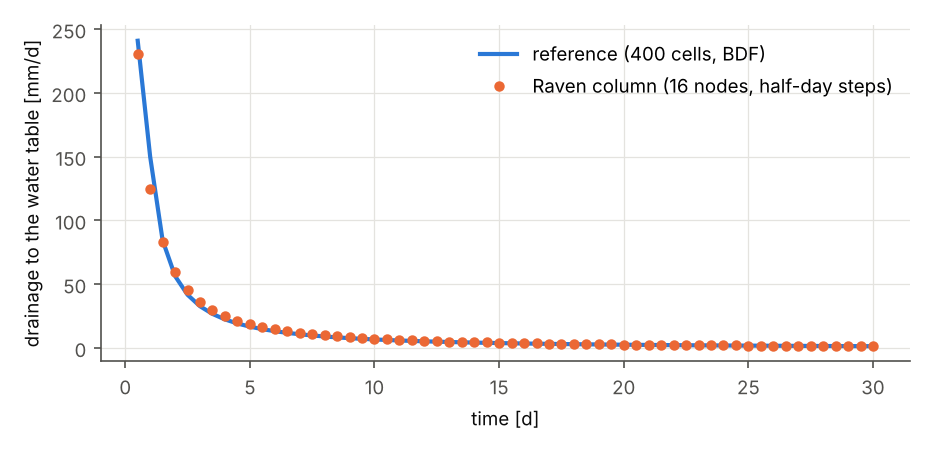
\includegraphics[width=0.49\linewidth]{figures/fig_sz_drainage.png}\hfill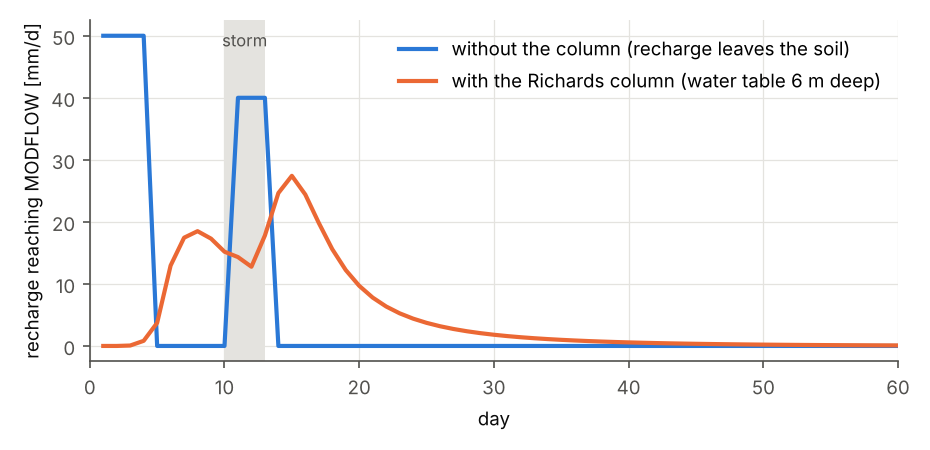
\includegraphics[width=0.49\linewidth]{figures/fig_sz_delay.png}
\caption{Left: drainage of a wet column to the water table, Raven's column against the reference solution
(step means). Right: recharge reaching MODFLOW after a 3-day storm with the water table 6~m deep
(test P1).}\label{fig:szdelay}\label{fig:szdrainage}
\end{figure}
\begin{figure}[!htbp]\centering
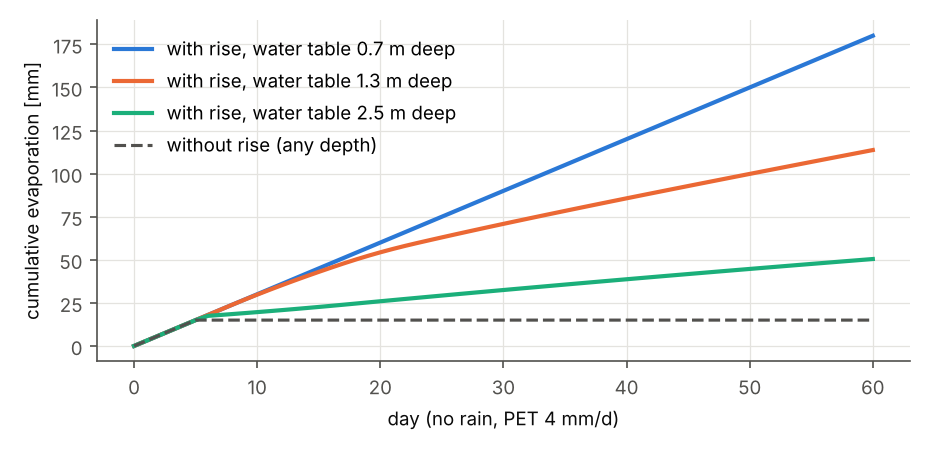
\includegraphics[width=0.49\linewidth]{figures/fig_sz_caprise.png}\hfill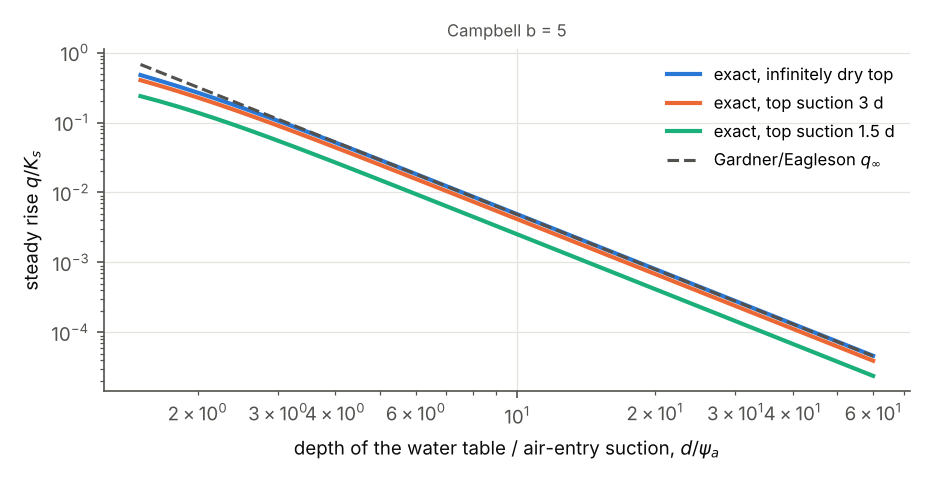
\includegraphics[width=0.49\linewidth]{figures/fig_sz_rise.png}
\caption{Left: evaporation from a drying soil over a shallow water table, with and without capillary rise (test P2).
Right: the steady rise from a water table (\ref{eq:rise}) for three suctions at the top, and Gardner's limit, which
overestimates the rise unless the soil is very dry.}\label{fig:szcaprise}\label{fig:szrise}
\end{figure}
\begin{figure}[!htbp]\centering
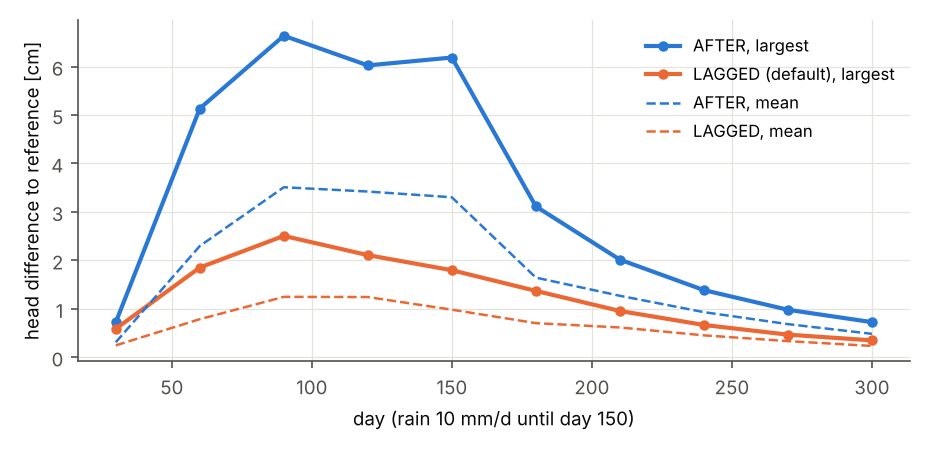
\includegraphics[width=0.56\linewidth]{figures/fig_sz_timing.png}\hfill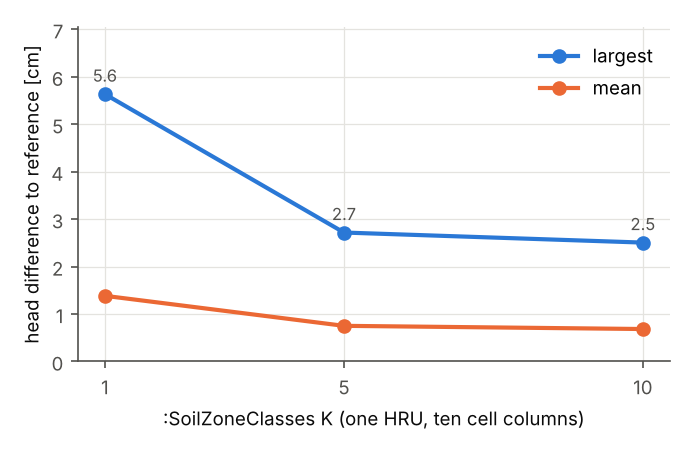
\includegraphics[width=0.42\linewidth]{figures/fig_sz_classes.png}
\caption{Left: head difference to the MODFLOW-only reference on the hillslope with the exchange after Raven's
processes (\cmd{AFTER}) and lagged (\cmd{LAGGED}, the default; test P5). Right: the same hillslope as one HRU, with Raven's
processes on 1, 5 and 10 classes of its columns (test P6).}\label{fig:sztiming}\label{fig:szclasses}
\end{figure}

\subsection{The interface iteration and MODFLOW's side}\label{sec:vszinterface}
Six scripts test the interface iteration, drained columns, heads far outside the model, negative recharge, MODFLOW's
budget as Raven books it and surface stores on soil-zone HRUs (Table~\ref{tab:vszinterface}; numbers of the quick mode, \cmd{RAVEN\_TEST\_QUICK=1}). The negative
recharge cases run in \cmd{test\_robustness.py} as R14--R22.
\begin{longtable}{P{0.13\linewidth}P{0.42\linewidth}P{0.36\linewidth}}
\caption{The interface and MODFLOW's side (\cmd{test\_interface\_stiff}, \cmd{test\_confined\_wet}, \cmd{test\_columns\_mf6},
\cmd{test\_robustness} R14--R22, \cmd{test\_mf6\_budget}, \cmd{test\_surface\_stores}).}\label{tab:vszinterface}\\
\toprule\hdr Test & Case & Result\\\midrule\endfirsthead
\caption[]{The interface and MODFLOW's side (continued).}\\
\toprule\hdr Test & Case & Result\\\midrule\endhead
S1 & low-$K_v$ top layer ($K_v$ 0.5~mm/d), wet spell from 3~m deep; columns from 1.5~m & every step converged; 4.0 (NONE) and 5.9 (RICHARDS) outer iterations per step; $F$ up to 1, column inflow 6\,530~m$^3$\\
S2 & $S_y$ 0.02, one base point per cell, rising water into a drying soil (kink drain) & converged; 4.4 / 6.0 outer iterations per step\\
S3 & explicit coupling over a 0.8~m top layer, egg-crate slope, specified head & no shortfall\\
S4 & \cmd{:SoilZoneIteration} 1 and 2 & 400 / 20 (NONE) and 400 / 60 (RICHARDS) supply-limited updates; largest take beyond the free water $2\cdot10^{-13}$~m$^3$/d\\
S5 & S4 with constant percolation and PET 5~mm/d from 1~m & take $2\cdot10^{-13}$~m$^3$/d\\
S6 & outer-iteration limit 1, iteration 0 and 1 & explicit; outputs identical\\
S7 & limits 2 and 3 & 6 of 10 steps converged (those without exchange); no ``no change \ldots to compare with''\\
S8 & connection test: stored case lowkv\_g57 without rain, $d_s$ 0.5~m, 16~m deep, head tolerance 0.05~m; default limit and limit 20 & 1 drop, its next update plain; with limit 20 the warning names the connection test at HRU 1, cell (1 1 6), fraction 0.0027 against 0\\
W1--W3 & confined layer below its bottom, generated and existing (ICELLTYPE from memory) & every step converged, no column kept wet\\
W5 & case Dc (existing, ICELLTYPE 1/0/1, ICONVERT 1, 20\,\% slope, dry then 30~mm/d) & 43 of 43 steps, 0 unconverged\\
W7 & confined model with a 10$^4$~m$^3$/d well, far heads that converge; W7c limit 3 & warned once; W7c completes, 8 MODFLOW-unconverged steps carried on, pumped head within 0.9\,\% of the default run, every warning's percentage equal to GWBudget's\\
W9, W10 & the same with limits 2 and 1 & stop: residual 2\,\% of the gross flow / the solve moved the head 1\,241~m; messages name head, cell (1 2 2), residual and causes\\
W12 & existing model with an inactive top layer, limit 2 & every interface warning names layer 2\\
W13 & the W7 model generated, \cmd{:SolverMaxOuterIterations 3} (steps 1--8 unconverged): restarts after unconverged steps & \cmd{:GWStartHeads} written after day 3 and carried unchanged through a restarted unconverged day, none after a converged day; a restart on day 4 equals the continuous run (difference 0)\\
M1--M4 & drained columns kept wet; a column delivers its inflow; \cmd{CONCEPTUAL} against a reference build; missing summary line & kept in 5 outer iterations; outflow 1.02 of the inflow; byte-identical except the balance-error \%\\
R14--R20 & negative recharge (\cmd{PERC\_GR4JEXCH}): split, cut by the top cell, hand-back, not held, existing model without \cmd{NEWTON} (confined variant), column upflow, sibling columns & identities at round-off; cut 437\,045~m$^3$; not held 3\,793 (LAGGED) / 2\,870 (AFTER)~m$^3$; not applied $-408\,000$~m$^3$, 0 with confined cells; not held only where the HRU's soil is empty (334~m$^3$)\\
R21 & a step with negative recharge in which wet unsaturated columns vanish under a water table raised by a specified head (\cmd{RICHARDS}; \cmd{KINEMATIC} in the full mode) & the vanished columns' water beyond $S_y\,\Delta h$ goes back to the soil zone as the link's rejected recharge; recharge identity 0\\
R22 & negative recharge with three depth classes, the hollow classes without a column (\cmd{RICHARDS}; \cmd{LAG} in the full mode) & MODFLOW's recharge on step 1 equals the top-cell limit (ratio 1.000000, as with one class); the cut, 2\,620~m$^3$, back to the soil zone\\
SW1--SW3 & \cmd{:SurfaceWaterExchange} on \cmd{DEPRESSION} of \cmd{:SoilZone PHYSICAL} HRUs, generated and existing model; a control with the water table above the ground at the outlet & stores' bed at the ground (model top + 1.0~m of soil zone); no discharge into the stores while every water table is below the ground; leakage 6\,135~m$^3$; existing model within $5\times10^{-6}$; control: discharge 1\,399~m$^3$\\
SW4 & restart of the control after 10 days, with a depression filled by groundwater to 64.6~mm (\cmd{DEP\_MAX} 50~mm) & the store is kept, not clipped to its maximum: Depression and the discharge into the stores equal the continuous run ($2.5\times10^{-9}$; a clip to the maximum would lose 583~m$^3$ and put the discharge 9\,\% off)\\
B1--B7 & steady existing model without STO (converged and OUTER\_MAXIMUM 3), gross flow, hourly dates, specified head under a dry cell, \cmd{:SoilZoneClasses 3}, audit guard counts & balance error $6\cdot10^{-12}$; residual equals the list file's IN$-$OUT within $1.3\cdot10^{-8}$ of the gross flow; gross flow equals TOTAL IN$+$TOTAL OUT within $5\cdot10^{-10}$; dates with times; warning names 2 columns over specified heads; no round-off as not held; guard counts 12 and 2\\
B8 & without \cmd{:SoilZone PHYSICAL}, \cmd{:SolverMaxOuterIterations} 2 (10 unconverged steps) and 1 (every step), and the Liard example (rivers and lakes) at 2: each row's residual over all its columns equals MODFLOW's negative residual on unconverged steps and 0 otherwise; run total ``discharge withheld''; at most ten warnings & step 1: 1\,039.4~m$^3$/d withheld = $-$balance error; run total 1\,062.5~m$^3$ = sum of rows; limit 1: 18\,511~m$^3$; 10 warnings (full mode)\\
B9 & \cmd{GWSoilExchange.csv} against \cmd{GWBudget.csv}: a generated model with an HRU wholly over specified-head cells, an existing model with a specified-head toe & on every date the four exchange columns summed over the HRUs equal \cmd{GWBudget.csv}'s within $2\cdot10^{-10}$ of the gross flow; the HRU over specified heads reports its base and water table\\\bottomrule
\end{longtable}
\noindent W4, W6 and W11 are reported as skipped: W4's rough-terrain cases run in \cmd{test\_rough\_terrain.py}; W6 (the
far-head warning once per ensemble member) and W11 (a head crossing the model) are not implemented as tests.

\subsection{Unsaturated-zone methods, depth classes and steady starts}\label{sec:vszmethods}
The \cmd{KINEMATIC} and \cmd{LAG} methods and the depth classes have their own tests, described with each method:
\cmd{test\_vz\_kinematic.py} K1--K9 (Section~\ref{sec:szvadosekw}), \cmd{test\_vz\_lag.py} LU, L1--L7, LS and the byte-identity
check LB (Section~\ref{sec:szvadoselag}), and \cmd{test\_vz\_classes.py} C1--C11 (Section~\ref{sec:vzclasses}). Among the
latter, C9 runs the rough-terrain case RT20 (stored existing model e43, \cmd{LAG}) with three depth classes through
\cmd{test\_rough\_terrain.py}: the saturated fraction stays within 0.0001 of the closure (limit 0.004) and no run fails; C10
writes a hotstart after a step that dropped a class column ($K=3$; after 4, 10 and 13 days): no mismatch warning, and the
restart within $7.5\times10^{-7}$ of the continuous run. \cmd{test\_vz\_initial.py} checks the steady start of
\cmd{:SoilZoneVadoseInitialFlux} (Section~\ref{sec:szvadose}):
\begin{itemize}
\item VI1, VI2, VI4: columns started at the steady profile carry their flux from the first step, with the storage at the start
in \cmd{GWModelSummary.txt}; hotstarts restore the columns; the columns' balance closes from step 1;
\item VI5: the steady start is for the flux each column receives, $(1-F)\,q$ (hummocks $\pm3$~m, water table 3~m deep,
$F=0.16$, 2~mm/d, \cmd{RICHARDS}, \cmd{KINEMATIC}, \cmd{LAG}, $K=1$ and 3): step-1 outflow = inflow = 100.8~m$^3$, 25.6~m$^3$
rejected;
\item VI6: a column that cannot carry $q$ (\cmd{K\_VERT} 1~mm/d under 2~mm/d) starts backed up: storage unchanged, outflow =
inflow = 40.000~m$^3$, 40.000 rejected, with a warning;
\item VI7: a restart with \cmd{:SoilZoneVadose NONE} from a file holding columns (\cmd{LAG}, $K=3$, negative recharge, 4 days):
a warning names the columns and their water, and \cmd{GWModelSummary.txt} reports it (248~m$^3$, the first run's final
unsaturated storage);
\item VI8: a restart with \cmd{:SoilZoneSubgrid 8} from a file written with 5 (\cmd{RICHARDS}, $K=3$): the columns' tops differ,
so they start at rest with a warning (0 against 5.37~m$^3$ written); with \cmd{:SoilZoneSubgrid 5} the written water is read exactly;
\item VI9: a restart with another method (the column case, $K=1$): written by \cmd{RICHARDS} and read by \cmd{KINEMATIC}, and
the other way round, the columns start at rest, the warning names the writing method and the run total reports the
first run's final storage (3.72 and 491~m$^3$; read as the other method's contents they would start with $+3\,669$ and
$-3\,628$~m$^3$); \cmd{RICHARDS} read by \cmd{LAG} starts with the written water;
\item VI10: a restart with a specified head added over HRU~1 (\cmd{LAG}, $K=1$, initial flux 30~mm/d): the 2 lines on its
cells are not used, and the warning and the run total give their 77.5~m$^3$ (start storage plus that volume equals the
file's water);
\item VI11: a generated model whose \cmd{:BoundaryHead} series holds the outlet cells at the start builds no column on them
(start storage 839.0~m$^3$, as with a fixed head; built there, the columns would ship 120~m$^3$ of initial-flux water to
the specified heads in step 1);
\item VI12: columns over an existing model's own specified heads (\cmd{KINEMATIC}, $K=3$, periods 3--5): a restart on day 4
rebuilds them at rest and ends them again, but only columns that held water are counted, so the two parts' run totals
add up to the continuous run's (18 columns, 225.75~m$^3$);
\item VI13: a generated model's \cmd{:BoundaryHead} series below the aquifer on days 1--3 (columns form on its cells) and
near the ground from day 4, restarted from day 3's \cmd{solution.rvc} (\cmd{LAG}, $K=1$; \cmd{KINEMATIC}, $K=3$,
\cmd{LAGGED}): the restart builds those columns from the file and ends them in its first step, so \cmd{GWBudget.csv} from
day 4 equals the continuous run's (deviation 0; day 4's recharge onto the specified heads 51.79 and 94.32~m$^3$/d).
\end{itemize}

\subsection{Input handling}\label{sec:vszinputs}
\begin{longtable}{P{0.07\linewidth}P{0.55\linewidth}P{0.30\linewidth}}
\caption{Soil zone and hotstarts: input handling (\cmd{test\_inputs.py}; short runs of the CT1 column unless stated).}\label{tab:vszinputs}\\
\toprule\hdr Test & Case & Result\\\midrule\endfirsthead
\caption[]{Soil zone and hotstarts: input handling (continued).}\\
\toprule\hdr Test & Case & Result\\\midrule\endhead
I1 & \cmd{HYDRAUL\_COND} missing for the soil class of the bottom soil-zone layer & stops (``needs HYDRAUL\_COND'')\\
I2 & \cmd{:SoilZoneIteration} with the update count only (0) & accepted; explicit, no interface update\\
I3 & \cmd{:SoilZone PHYSICAL} followed by \cmd{:SoilZone CONCEPTUAL} & the last counts: a conceptual run\\
I4 & soil-zone options under \cmd{CONCEPTUAL} & reported as ignored\\
I5 & a \cmd{:GWSoilZoneColumns} block with a column missing & reported (``do not match its soil-zone columns'')\\
I6 & the same block with its rows in another order & used (matched by cell)\\
I7 & groundwater blocks in the \cmd{.rvc} of a run without \cmd{:GroundwaterModel} & skipped; Raven's initial conditions after them apply\\
I8 & \cmd{:SurfaceWaterExchange} on a soil-zone layer & refused\\
I9 & a damaged \cmd{:GWHeads} header (\cmd{-1 2 2}; \cmd{100000 100000 100000}) & stops with a message\\
I10 & \cmd{:StartTime} in the \cmd{.rvc}, run under valgrind & no uninitialised read in \cmd{ParseInitialConditionsFile} or \cmd{TimeDifference}\\
I11 & \cmd{:BoundaryHead NOPE} beside boundary \cmd{EDGE}; \cmd{:WellFlowRate 7} with only well 1 & stop naming the series and the boundaries or wells there are; the right names run\\
I12 & \cmd{:SeepageToRaven}, \cmd{:KeepPackages}, \cmd{:MF6StartDate}, \cmd{:MF6Model} on a model Raven builds; depth classes and initial flux with \cmd{NONE}; \cmd{:SoilZoneAquiferClass} on a generated model; an unknown profile attribute; \cmd{LAYERS BOTTOM} & the four stop; the next three are reported as ignored; the last two stop\\
I13 & a missing \cmd{.rvg} file; a short \cmd{:Wells} row & named in \cmd{Raven\_errors.txt}; the message names \cmd{:Wells}\\
I14 & age tracer (no groundwater): 20 days against 7 + 7 + 6 days chained through \cmd{solution.rvc} & ages of every store and the outflow within $2\times10^{-4}$~d plus $10^{-5}$ of the age (the six digits of \cmd{Ages.csv}) of the continuous run, largest difference $10^{-4}$~d; \cmd{:StartTime} the start of each part, \cmd{:AgeTracerDatum} 2000-01-01 in the restarted parts\\
I15 & age-tracer chains across year boundaries: 1999-12-25 (7 + 7 + 6 days), 1998-12-20 (400 + 380 days; quick mode 12 + 400 + 8) & every part runs; ages within the limit of I14, largest difference $10^{-4}$~d; \cmd{:AgeTracerDatum} 1999-12-25 and 1998-12-20\\
I16 & age tracer started from the \cmd{solution.rvc} of a 30-day spin-up without it & ages 0 at the start, 1~d after the first day; no \cmd{:AgeTracerDatum}\\
I17 & EnKF, 3 members, one well, \cmd{:ExtraRVTFilename} with $-100$, $-200$, $-300$~m$^3$/d & each member pumps its own rate; a series naming no well stops the run\\
I17b & EnKF, 2 members whose \cmd{:ExtraRVTFilename} gives a \cmd{:BoundaryHead} series (99~m, then 70~m below the aquifer) to a specified head the base \cmd{.rvt} leaves fixed & each member's model is built with its series: the cells are released on days 3--6, nothing is booked onto them, and both members' \cmd{GWBudget.csv} equal the single run with the series in its \cmd{.rvt}\\
I18 & \cmd{:GWSoilZoneColumns} with \cmd{nan} or $-50$~mm, \cmd{:GWHeads} with \cmd{nan} & each stops with a message naming the block; the undamaged file runs\\
I19 & \cmd{:Transport Nitrate} (\cmd{CONCEPTUAL}, \cmd{PHYSICAL}) and \cmd{:Transport AGE} with \cmd{:GroundwaterModel MODFLOW6}; the same model without groundwater & the coupled runs stop naming the constituent; the run without groundwater completes\\
I20 & a specified head with \cmd{HEAD} 0 (below every cell) and a \cmd{:BoundaryHead} series of 99.5~m; the same without the series & placed by the series: 2 cells, flow 1\,390~m$^3$; without it no cell and a warning naming the boundary, its head and the highest cell bottom\\
I21 & head boundary \cmd{EDGE} (\cmd{HEAD} 90) with a series of 99~m on day 1, then 90~m; layer 1 from 100 to 97~m: (a) a GHB (\cmd{LAYERS TOP}) against an aquifer at 95~m; (b) a CHD (\cmd{LAYERS TOP}); (c) a CHD (\cmd{LAYERS ALL}, 99~m for 3 days), restarted on day 4 & (a) the GHB drains on days 2--6 ($-7\,915$ to $-2\,275$~m$^3$/d), as with \cmd{HEAD} 90 alone; a series of 90~m gives the outputs of \cmd{HEAD} 90; (b) the water table falls below 97~m (93.8 to 92.9~m): no cell is held at the bottom of layer 1; (c) the restarted run has the same 4 CHD cells and the same flows and heads as the continuous run\\
I21 (d) & a column with no cell held: 8 HRUs, the last wholly on \cmd{EDGE} (\cmd{LAYERS ALL}), rain 20~mm/d, a series of 99~m on days 1--2 and 70~m (below the aquifer) on days 3--6; \cmd{CONCEPTUAL} and \cmd{PHYSICAL} & days 3--6: CHD flow 0 and nothing booked onto specified-head cells; MODFLOW's recharge equals Raven's (\cmd{CONCEPTUAL}); the column's soil-zone link exchanges 425 to 42~m$^3$/d with the aquifer (\cmd{PHYSICAL}); every identity holds\\
I21 (e) & \cmd{LAYERS TOP}, \cmd{HEAD} 90 and a series of 99~m on every day, CHD and GHB & the cells of layer 1 only (2), none switched off\\
I21 (f) & a steady-state first period at 90~m (series 90, 99, 99, 90, 90, 99~m) & the run total counts the steady period's 2 cells: 8 cell-steps against 6 without it\\
I22 & \cmd{:InitialGWHeads ELEVATION 98,5}, \cmd{H98.5}, \cmd{0x62}, \cmd{98.5}, \cmd{98.5\# note} and \cmd{98.5 \# note}; \cmd{:InitialGWHeads FROM\_PROFILE 0}; a \cmd{:GWHeads} value \cmd{98.1x} & the first three stop naming the command and the token (surplus value '5'; not a number), the next three start at 98.5~m; \cmd{FROM\_PROFILE 0} stops (takes no value); the damaged value stops naming the block\\
I23 & two \cmd{:SpecifiedHeadBoundary} commands on the same file (\cmd{HEAD} 99 and 99.5); two \cmd{:GeneralHeadBoundary} commands on it & the first stops before MODFLOW starts, naming both boundaries and the cell; the second runs\\\bottomrule
\end{longtable}

\subsection{Robustness}\label{sec:vszrobust}
\begin{longtable}{P{0.07\linewidth}P{0.55\linewidth}P{0.30\linewidth}}
\caption{Soil zone: robustness (\cmd{test\_robustness.py}; hard cases of the interface). R14--R22, the negative-recharge
cases, are in Table~\ref{tab:vszinterface}.}\label{tab:vszrobust}\\
\toprule\hdr Test & Case & Result\\\midrule\endfirsthead
\caption[]{Soil zone: robustness (continued).}\\
\toprule\hdr Test & Case & Result\\\midrule\endhead
R1 & stiff flat column: drainable porosity 0.02 against $S_y=0.25$, high conductance & every step converged; at most 12 updates, 27 outer iterations\\
R2, R2c & one HRU over ten cells against ten one-cell HRUs; R2c with constant-rate percolation & outflow $-0.2\,\%$, MODFLOW recharge ratio 1.00; R2c outflow $-0.2\,\%$\\
R3 & \cmd{RECHARGE\_DELAY} with \cmd{:SoilZone PHYSICAL} & refused\\
R4 & a smoothing depth below 0.1~m & warned\\
R5 & hourly steps, smoothing depth 0.001~m & no unconverged step; MODFLOW error $1.1\times10^{-11}$\\
R6 & slope 0.1 with $5\times5$ DEM points per cell & converged; at most 8 updates\\
R7 & explicit mode (\cmd{:SoilZoneIteration 0}) & no shortfall\\
R8 & one column $10^{-6}$~mm wetter than the others & heads stay uniform ($3.7\times10^{-9}$~m)\\
R9 & hotstart columns that cannot hold the \cmd{.rvc} layer split & 4\,000~m$^3$ redistribution reported in step 1, 0 later\\
R10 & water rising into a thin soil on a steep, low-storage slope, update budget 1 and explicit mode & no shortfall\\
R11 & explicit mode on the R2 hillslope against the iterated run & outflow within 0.6\,\%\\
R12 & explicit mode, 15 outer iterations, water rising into cells dry at the head of linearization & converged; outflow within 0.6\,\%; MODFLOW error $10^{-7}$\\
R13 & stiff low-storage slope, budget 1, 12 outer iterations, MODFLOW unconverged & neither residual nor shortfall handed to Raven: outflow 1.01 times the iterated run's\\
R15b & a negative-recharge cut on a draining soil zone: 8.67~mm cut while the wet soil drains & soil zone after step 1 at least its field-capacity water (126.08 against 120~mm)\\\bottomrule
\end{longtable}

% Verification on rough terrain (tests/soilzone/test_rough_terrain.py, rough_models.py, rough_ext.py, rough_cases/).
\section{Rough terrain}\label{sec:vrough}
The tests of Section~\ref{sec:vsoilzone} use planar hillslopes. Real ground is irregular: slopes change within a cell,
the land holds pits, closed depressions, cliffs and ridges, the DEM is finer or coarser than the grid and may end inside
it, and the MODFLOW layers slope, thin out and pinch against bedrock. The rough-terrain suite
(\cmd{tests/soilzone/test\_rough\_terrain.py}) draws such cases at random from a seed, runs each with every
unsaturated-zone method and checks every run against rules that hold whatever the ground looks like. A seed always gives
the same case, so every failure can be replayed (\cmd{--case}).

\subsection{What the cases vary}
Every fourth seed couples an existing MODFLOW~6 model written by the suite (\cmd{rough\_ext.py},
Section~\ref{sec:vexisting}); the others let Raven build the model (\cmd{rough\_models.py},
Section~\ref{ch:layers}). Table~\ref{tab:vroughvary} lists the ranges.
\begin{table}[!htbp]\centering
\caption{What the rough-terrain cases vary (\cmd{rough\_models.gen\_spec}; existing models: \cmd{rough\_ext.ext\_spec}).}\label{tab:vroughvary}\small
\begin{tabular}{P{0.2\linewidth}P{0.74\linewidth}}\toprule\hdr
Item & Range\\\midrule
ground & a plane sloping 0--30\,\% in any direction plus roughness: spectral noise, bumps, pits, closed depressions, cliffs (steps a few metres wide, or sharper than the DEM) and ridges; relief within a cell from 0.05 to 6 times the soil-zone thickness $D$\\
DEM & resolution 0.08--1.6 cells; NODATA holes; a DEM that ends inside the grid (cells partly without land samples)\\
grid and HRUs & cells of 25--150~m, 4--9 by 3--6 cells; a tiling of HRUs cut at random positions (on and off cell edges, one-cell HRUs); domain edges on or inside cells; \cmd{:MinCellCoverage} 0.1--0.5\\
soil & two soil profiles by position, two layers, $D$ 0.3--3~m; Campbell retention for the capillary rise; \cmd{PERC\_CONSTANT} or \cmd{PERC\_GAWSER\_CONSTRAIN}\\
aquifer (generated) & two aquifer profiles by position, 1--3 layers of 2--3 classes ($K_h$ 0.05--30~m/d, $K_v$ down to $10^{-2.5}K_h$, $S_y$ 0.02--0.3, retention for the columns); thin layers (0.2--0.8~m); sloping bedrock raster (or \cmd{DEFAULT\_BEDROCK\_DEPTH}), so layers slope, pinch out, are clipped at bedrock and become pass-through cells; bedrock at least $\max D+1.0123$~m below the land, except in outcrop cases (bedrock above the soil-zone base under a whole HRU)\\
aquifer (existing) & DIS or DISV (irregular quadrilaterals); top = mean land $-D$, moved up or down by up to $D$; 1--3 layers whose thicknesses tilt across the model, pass-through cells (\cmd{IDOMAIN}~$-1$) where a layer thins below 0.5~m, inactive columns and columns with an inactive first layer (\cmd{IDOMAIN}~0); a confined bottom layer in some models; \cmd{NEWTON} in most models, a few without it\\
water & \cmd{:SoilZoneSubgrid} 1, 3, 5, 9; \cmd{SEEPAGE\_SMOOTHING\_DEPTH} 0.02--0.5~m; 40--90 daily steps; mean rain 8--45~mm/d on 10--40 wet days (daily 2.4--77~mm/d) between dry spells; soil evaporation 0--4~mm/d; start deep (3--15~m), shallow (0.2--2~m) or at the land; a specified head along the low edge; \cmd{:SoilZoneCapillaryRise} on, off or default; \cmd{:SoilZoneExchangeTiming} \cmd{LAGGED} or \cmd{AFTER}\\
\bottomrule
\end{tabular}
\end{table}

\subsection{What every run is checked for}
\begin{description}
\item[Run] The run completes, or stops with a justified message (below).
\item[Finite] No NaN or Inf in any output table, no non-finite head, no \cmd{HDRY} head in an active cell under \cmd{NEWTON}.
\item[Balances] The identities of Section~\ref{sec:audit} close within the standard limits (recharge $5\times10^{-9}$,
soil zone and unsaturated zone $10^{-8}$, MODFLOW $10^{-5}$ of the recharge, Raven $10^{-5}$~mm), and no soil-zone
shortfall is booked on a step whose interface converged.
\item[Layers] For generated models, \cmd{TOP}, \cmd{BOTM} and \cmd{IDOMAIN} as MODFLOW read them equal an independent
construction from the DEM, the bedrock raster and the profiles (Section~\ref{ch:layers}) within $10^{-6}$~m.
\item[Bases] The soil-zone base of every HRU equals the overlap-weighted land surface of its cells less $D$ (existing
models: the top of the top active cell).
\item[Saturated fraction] With \cmd{:SoilZoneVadose NONE}, the saturated fraction of every HRU equals an independent
closure --- the cell's DEM samples less $D$, none below 1~mm above the top cell's bottom, smoothed over $d_s$ --- at a head
between the top cells' heads at the start and the end of the step, on every converged step, within 0.02. With a column
method the difference is reported only: the fraction reported for a link whose column carries the step is the
connection's, not the one that rejected the recharge.
\item[Physics] $0\le F\le1$; soil water within $[0,$ capacity$]$; rejected recharge and overflow $\ge0$; with
\cmd{NONE} the rejected recharge is at most the HRU's recharge, positive only where $F>0$, and $F$ times the recharge on
HRUs over one cell; with a column method the rejected recharge of a step is at most its recharge plus the columns'
storage at its start.
\item[Heads] With a column method, no water table more than 5~m above the highest land sample of its cell, unless the
\cmd{NONE} run of the same case lifts it to within 1~m of that height.
\item[Convergence] Steps on which MODFLOW or the interface did not converge are counted; more than 5\,\% fails the case.
\end{description}
A run whose failures are all known ones is reported as a known failure (XFAIL): the suite keeps one known pattern, an
interface left unconverged where the land lies below the top cell's bottom, and no open case. A shortfall is never a known
failure, and a regression case's own checks are added before this is decided: any other failure makes the run fail.

\paragraph{Justified stops.} A run may stop without failing in three situations: an outcrop case (\emph{HRU \dots\ does
not overlap any active groundwater cell}); an existing model without \cmd{NEWTON} (\emph{:SoilZone PHYSICAL needs an
existing model that uses the Newton-Raphson formulation}); and a diverged solve (\emph{heads are not finite}, or a head
far outside the model on an unconverged step) that MODFLOW~6 repeats on its own. For the last, the suite runs the case's
MODFLOW model through the library without Raven's packages, with a drain at the top of every column as the only outlet
and no recharge, for the run's duration; the stop is justified only if those heads become non-finite or move by more
than $10^6$~m within the outer iterations. A column held 1~mm above its bottom (Section~\ref{sec:drained}) is reported,
not a failure.

\paragraph{Regression cases.} Twenty cases run first (RT1--RT20, Table~\ref{tab:vroughprob}): RT1 is a flat hillslope (the
configuration of P3 without columns) on which the rejection must follow the converged head: with the saturated fraction of
an earlier iterate it would reject 15\,\% of the recharge where the closure at the step's heads allows at most 5\,\%;
RT2--RT20 are stored cases (\cmd{rough\_cases/*.json}, each with its spec and the meta data the checks use) of the hardest
situations the suite draws. Each has
its own checks besides the above: RT6, RT11--RT13 and RT19 must complete (no stop at all), and RT20 (stored existing model e43,
\cmd{LAG}) must hold the saturated fraction to the closure within 0.004 with any method: its land lies in
places within the 1~mm band above the top cell's bottom, where no sub-grid base may lie. \cmd{--case} applies these checks
too when it replays a stored case.

\subsection{Results}
Table~\ref{tab:vroughres} summarizes the suite's 400 default seeds run with each of the four methods
(\cmd{--methods NONE,RICHARDS,KINEMATIC,LAG}, 1\,620 runs with the regression cases; the script's default runs
\cmd{NONE} and \cmd{RICHARDS} only). No run failed and none was a known failure. Every run that completed (1\,567 of
1\,620) closed all balances within the limits above (largest values: recharge identity $4.5\times10^{-10}$, soil-zone
identity $9.9\times10^{-10}$, unsaturated-zone identity $4.6\times10^{-10}$, MODFLOW $7.7\times10^{-6}$ of the recharge,
Raven $10^{-11}$~mm; largest shortfall $4\times10^{-14}$). The independent geometry agreed everywhere: layers to
$5\times10^{-8}$~m, bases to $5\times10^{-8}$~m. On converged steps the saturated fraction agreed with the closure to
0.0022 with \cmd{NONE} (limit 0.02); with a column method it is reported (largest difference 0.0027 with \cmd{RICHARDS}
and \cmd{LAG}, 0.0020 with \cmd{KINEMATIC}).
\begin{table}[!htbp]\centering
\caption{Rough-terrain suite, default seeds and regression cases, one depth class.
Run times depend on the machine and its load (two cores shared with another test suite).}\label{tab:vroughres}\small
\begin{tabular}{P{0.36\linewidth}P{0.13\linewidth}P{0.13\linewidth}P{0.13\linewidth}P{0.13\linewidth}}\toprule\hdr
 & \cmd{NONE} & \cmd{RICHARDS} & \cmd{KINEMATIC} & \cmd{LAG}\\\midrule
runs & 407 & 408 & 401 & 404\\
completed / justified stops & 393 / 14 & 395 / 13 & 388 / 13 & 391 / 13\\
known failures / failures & 0 / 0 & 0 / 0 & 0 / 0 & 0 / 0\\
time steps of completed runs & 25\,753 & 25\,809 & 25\,350 & 25\,528\\
steps with the interface unconverged & 0 & 0 & 0 & 0\\
steps with MODFLOW unconverged & 0 & 0 & 0 & 0\\
runs with the water table $>5$~m above the land; largest & 44; 94.2~m & 43; 94.2~m & 40; 94.2~m & 42; 94.2~m\\
MODFLOW outer iterations per step (mean) & 6.34 & 5.83 & 5.70 & 7.20\\
mean run time [s] & 0.16 & 0.22 & 0.18 & 0.19\\\bottomrule
\end{tabular}
\end{table}
The justified stops are the outcrop cases (g14, g33, g58, g61, g162, g223, g266), the existing models without
\cmd{NEWTON} (e36, e96, e200, e256, e316, e356: 6 of the 100 existing models, the others use it; with \cmd{NONE} also
the regression case RT17, which tests this stop), and stops that MODFLOW alone repeats (none). The run counts differ
between the methods because the regression cases run with one method each. Water tables far above the land occur where
the land is steep and the top layer's vertical conductivity low: the largest, 94.2~m, is seed g274 (slope 16\,\%,
150~m cells, $K_v=0.0047$~m/d) with every method, \cmd{NONE} included, so it comes from the aquifer model, not from the
columns (\cmd{--case 274}). No column method lifts such a water table over \cmd{NONE}'s (largest difference 0.0~m at
the 0.1~m resolution of the report); the column methods have fewer such runs than \cmd{NONE}. With
\cmd{:SoilZoneVadoseClasses 3} (\cmd{--vzclasses 3}, the same 1\,620 runs) the suite gives 0 failures and 0 known
failures, with the same completed runs and justified stops, no unconverged step, the same balance limits (largest
MODFLOW identity $8.3\times10^{-6}$), 0.0031 as the largest reported difference of the saturated fraction (\cmd{LAG}),
44, 43, 41 and 43 runs (\cmd{NONE}, \cmd{RICHARDS}, \cmd{KINEMATIC}, \cmd{LAG}) with the water table more than 5~m above the land (largest 94.2~m, g274, as
with one class; the column methods lift it by at most 0.1~m over \cmd{NONE}'s), 5.72, 5.61 and 7.13 outer iterations per
step (\cmd{RICHARDS}, \cmd{KINEMATIC}, \cmd{LAG}) and mean run times of 0.34, 0.22 and 0.23~s. RT20 holds the closure to
0.0001 with three classes (0.0002 with one class; limit 0.004). The water table of RT20's \cmd{LAG} run with three
classes differs from that with one class by at most 0.35~m: it is lower by up to 0.16~m during the first two weeks of the
rain (the upper classes' longer columns hold more of the rain on its way down), and higher by up to 0.35~m late in the
dry spell that follows the rain (day 67, as they release it).

\begin{table}[!htbp]\centering
\caption{The regression cases of the rough-terrain suite: the situation each one stores and the part of the coupling that
handles it. They run first in the suite.}\label{tab:vroughprob}\small
\begin{tabular}{P{0.44\linewidth}P{0.32\linewidth}P{0.15\linewidth}}\toprule\hdr
Situation & Handled by & Case\\\midrule
rejection on a converged step & the rejection follows the converged head & RT1\\
columns over cells filled to the soil-zone base & the columns' hand-back and the heads check & RT14--RT16\\
drained columns, which would leave MODFLOW's solve singular & a drained column is held 1~mm above its bottom once per step (and once more on any later solve in that step) & RT6, RT11--RT13\\
an existing model without \cmd{NEWTON} whose top cells dry & a start-up stop: \cmd{NEWTON} is required & RT17\\
\cmd{LAG} on a slowly permeable slope (g350), which must complete & the \cmd{LAG} cascade (Section~\ref{sec:szvadoselag}) & RT19\\
sub-grid bases in the 1~mm band below the lowest drain level & bases clipped at the top cell's bottom + 1~mm & RT3, RT20\\
the saturated fraction with three depth classes (a connection head away from MODFLOW's head) & the connection test (Section~\ref{sec:szinterface}) & RT20, also with three depth classes (C9)\\
slowly permeable or low-yield top cells, dried top cells, DISV models & head-dependent rejection, upward flow from a lower cell & RT2, RT4, RT5, RT7--RT10, RT18\\
\bottomrule
\end{tabular}
\end{table}

\begin{figure}[!htbp]\centering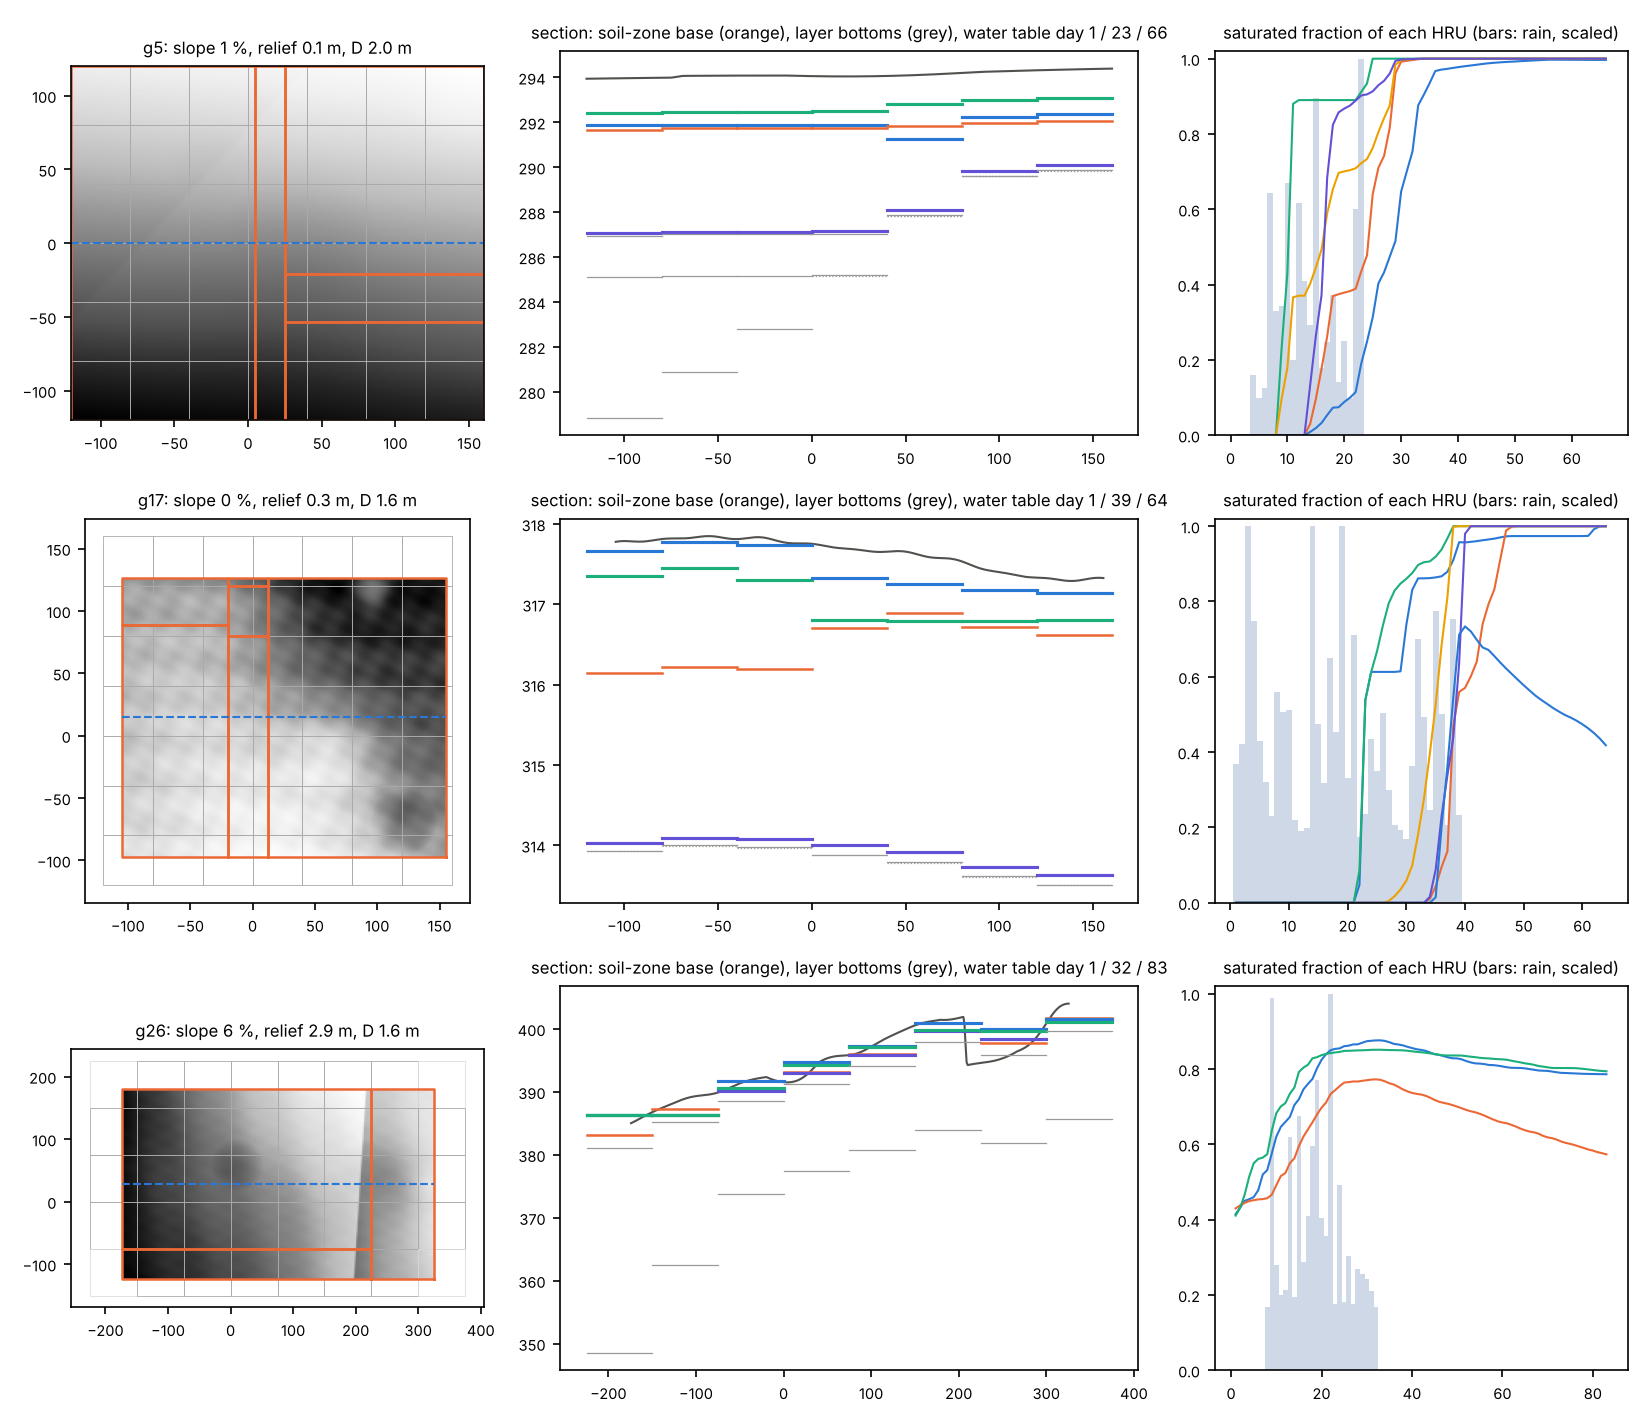
\includegraphics[width=\linewidth]{figures/fig_rough_cases.png}
\caption{Three cases of the suite (\cmd{:SoilZoneVadose NONE}). Left: DEM (shaded), grid cells and HRUs (orange); the
dashed line marks the section. Middle: land along the section, soil-zone base, MODFLOW layer bottoms of the cells it
crosses and the water table at the start, at the end of the rain and at the end of the run. Right: saturated fraction of
each HRU over the run.}\label{fig:vrough}
\end{figure}

\begin{refcard}{rough-terrain suite}
\begin{tabular}{@{}P{0.42\linewidth}P{0.53\linewidth}@{}}
\cmd{python3 test\_rough\_terrain.py} & regression cases RT1--RT20 and 400 seeds, \cmd{NONE} and \cmd{RICHARDS}\\
\cmd{--quick} / \cmd{--full} & 40 / 1\,500 seeds (\cmd{RAVEN\_TEST\_QUICK=1}: quick)\\
\cmd{--methods NONE,RICHARDS,KINEMATIC,LAG} & the methods run for every seed (and the regression cases whose method is listed)\\
\cmd{--vzclasses K} & \cmd{:SoilZoneVadoseClasses K} for every run\\
\cmd{--seeds a-b}, \cmd{--family gen|ext|both} & part of the seeds; generated or existing models only\\
\cmd{--case 57:RICHARDS}, \cmd{--case x43:LAG} & replay seed 57 (\cmd{x}: as an existing model); a column method is preceded by the case's \cmd{NONE} run\\
\cmd{--case rough\_cases/band\_e43.json:LAG} & replay a stored case with its own checks (or a run folder's \cmd{case.json}); the exit status is the run's\\
\cmd{--keep}, \cmd{--noreg} & keep the run folders; skip the regression cases\\
\end{tabular}
\end{refcard}


\section{Build checks}\label{sec:vbuild}
\cmd{tests/cmake\_checks.py} runs 22 offline configure checks of Raven's CMake integration of MODFLOW~6
(Section~\ref{sec:building}) in about a minute, without compiling Raven (Table~\ref{tab:vcmake}). \cmd{-{}-selftest} puts
the defect each check guards against back into a copy of the source and shows that the check then fails.
\cmd{tests/mf6version\_check.py} checks Raven's run-time version guard with a stand-in library, and
\cmd{tests/mf6lib\_check.py} how \cmd{tools/get\_mf6.py} chooses the release for each platform and where Raven finds the
library. The installed folder is checked by \cmd{cmake/RavenMF6InstallCheck.py}: it runs the installed Raven on a tiny coupled
model and checks that it used the library beside it and that every Fortran runtime library it loaded lies in that folder.

\begin{longtable}{P{0.07\linewidth}P{0.86\linewidth}}
\caption{CMake checks (\cmd{tests/cmake\_checks.py}).}\label{tab:vcmake}\\
\toprule\hdr Check & What is checked\\\midrule\endfirsthead
\caption[]{CMake checks (continued).}\\
\toprule\hdr Check & What is checked\\\midrule\endhead
1 & the default on Linux aarch64 without the source tools falls back to \cmd{OFF} with a warning naming \cmd{-DRAVEN\_MF6=OFF}; the configure succeeds\\
2 & that default survives a reconfigure and becomes \cmd{SOURCE} when the tools appear and the repository answers\\
3 & run path: the library from the build tree and from a moved install (\cmd{\$ORIGIN})\\
4 & \cmd{PATH} mode installs a symbolic link or a renamed library as \cmd{libmf6.so}\\
5 & \cmd{libmf6\_version.txt} and the package name (unknown for \cmd{PATH}, the \cmd{meson.build} version for zips and sources)\\
6 & offline options name their mode; options of another mode are reported as ignored; an unpinned zip is warned about\\
7 & meson gets the Fortran compiler of \cmd{FC}\\
8 & a meson whose version cannot be read is named as such\\
9 & a staged install (\cmd{DESTDIR}) gets \cmd{libgfortran.so.5}\\
10 & without git the default falls back, \cmd{SOURCE} stops naming git, and \cmd{RAVEN\_MF6\_SOURCE\_URL} needs none\\
11 & a replaced zip is unpacked again, an unchanged one is not\\
12 & Windows AMD64 and ARM64 (emulated)\\
13 & the package version from a \cmd{v6.7.2.tar.gz} source URL; an unpinned zip is ``not checked''\\
14 & a wrong \cmd{RAVEN\_MF6\_ZIP\_SHA256} stops the configure (local and downloaded zips)\\
15 & offline default: with the source tools but an unreachable git repository the default falls back at configure time to \cmd{PREBUILT} (a local release folder: the library target builds without network) or, with no release either, to \cmd{OFF} with a warning; a reachable repository gives \cmd{SOURCE}\\
16 & a single-configuration generator without \cmd{CMAKE\_BUILD\_TYPE} configures \cmd{Release} (\cmd{-O3 -DNDEBUG}); a given \cmd{Debug} is kept\\
17 & a MODFLOW version below 6.5.0 as \cmd{RAVEN\_MF6\_VERSION} (\cmd{SOURCE} and \cmd{PREBUILT}), in a zip's or a source folder's \cmd{meson.build} or in an archive name stops the configure naming 6.5.0; 6.7.0 configures with a warning naming 6.8.1\\
18 & runtime bundling, emulated on Linux: macOS with Mach-O stand-ins (\cmd{@rpath} chains resolved through \cmd{LC\_RPATH}, every reference rewritten to \cmd{@loader\_path}, every edited file signed); Windows with stand-in \cmd{objdump} and \cmd{dumpbin} (the DLLs \cmd{libgfortran-5.dll} imports installed)\\
19 & messages for a folder given as \cmd{RAVEN\_MF6\_PATH} and for a SHA-256 that is not 64 hex digits\\
20 & \cmd{PATH} mode on Linux: a gfortran-built library without a run path gets \cmd{\$ORIGIN} from \cmd{patchelf} and loads the runtime installed beside it; without \cmd{patchelf} a warning says that it loads the system's runtime; a library that has \cmd{\$ORIGIN} is left as it is\\
21 & \cmd{RAVEN\_MF6=OFF} (given, and as the default's fallback): the configure says that \cmd{cmake --install} installs Raven alone, and the install does so with a message\\
22 & the default's offline fallback to \cmd{OFF} with the source tools installed names the network; without meson the warning asks for the source tools\\\bottomrule
\end{longtable}
\noindent Real macOS and Windows systems are not part of these checks: the bundling there is emulated.

\section{Code checks}\label{sec:codeaudit}\label{sec:sanitizer}
\begin{itemize}
\item \textbf{Review:} line-by-line reading of the coupling's files and of every changed Raven file --- units, signs,
indices, order of operations, and that each volume is applied once on each side.
\item \textbf{Compilers and static analysis:} GCC and Clang, unoptimised and optimised: no warnings with \cmd{-Wall -Wextra
-Wshadow} in the coupling's files (with and without NetCDF); none from cppcheck and clang-tidy. A Windows build (MinGW) run
under Wine gives the Linux results to rounding.
\item \textbf{Sanitizers:} complete builds with AddressSanitizer and UndefinedBehaviorSanitizer, run on random set-ups covering
every option, an ensemble and a restart, on one random set-up of every grid type, on the faulty-input set-ups of
Section~\ref{sec:mf6files}, on seven reservoir and ensemble cases and on three years of the Liard model: no memory error and
no undefined behaviour. The only reported leaks are allocated inside the MODFLOW library.
\item \textbf{valgrind:} a hotstart with \cmd{:StartTime} (test I10, Table~\ref{tab:vszinputs}) reads no uninitialised value
in the hotstart code. valgrind reports uninitialised reads in two routines of Raven itself that the coupling does not touch
(Section~\ref{ch:limits}, known issues).
\end{itemize}

\section{Option combinations}\label{sec:vcombinations}
\cmd{tests/combinations.py} runs small synthetic models (four HRUs on a slope, 100~m cells) across a matrix of options and
checks every water identity on each run. The exchanges (water-table ET, a river, surface stores, a reservoir, a well, a
general-head and a specified-head boundary, each placed at the height of the ground where it lies) are combined all
together and one at a time; each under plain conditions, dry top cells (a 1~m top layer above the water table) and
negative recharge (\cmd{PERC\_GR4JEXCH}); with \cmd{CONCEPTUAL} and \cmd{:SoilZone PHYSICAL} (with
\cmd{:SurfaceWaterExchange} on the surface stores). The lake loses water where it lies on the ground (its stage above the
ground of its cells) and gains it as a pit lake half over the specified-head cells (its stage below the specified head);
water-table ET draws on a PET the soil cannot meet from a water table within the extinction depth. The unsaturated
columns (\cmd{RICHARDS}, \cmd{KINEMATIC}, \cmd{LAG}, one and three depth classes) run under negative recharge, a water table
rising through them (the columns vanish) and dry top cells. A boundary group switches cells off and on with
\cmd{:BoundaryHead} series (also every cell of a column, which is then an ordinary column) and switches an existing
model's own specified heads on under a lake. Every case except the \cmd{:BoundaryHead} series cases of the boundary group (6 in quick mode, 8 in full mode; generated model only) runs with the model Raven builds and as an existing model (with
\cmd{NEWTON}, without it for \cmd{CONCEPTUAL}, and converted to feet and seconds, the model's own river, well and boundaries
included). On every run: MODFLOW's balance, the recharge, soil-zone and unsaturated-column identities, Raven's balance, the
river, surface-store and reservoir books, the seepage returned, the run totals against their columns, and no HDRY or NaN in
the groundwater outputs. Every run must also move water through each exchange and stress its case names, and lists the
volumes moved: a case whose exchange moves none fails (in an existing model without \cmd{NEWTON} with dry top cells, which
MODFLOW takes out of its solve, the surface stores, the lake and the river must move none). The quick mode runs 311 runs
of 8 days (a few minutes), the full mode 393 runs of 15 days, with half-day steps too.
\cmd{tests/reservoir\_checks.py} checks the reservoir exchange where a lake's cells cannot all take seepage (existing and
generated models), its bed under \cmd{:SoilZone PHYSICAL}, and the run total of gains MODFLOW does not supply. One result is reported
apart as known: where a reservoir's stage falls back below its weir crest while groundwater feeds it, Raven's balance error
equals the reservoir routing's own balance error (a few m$^3$, \cmd{ReservoirMassBalance.csv}); the coupling's books hold.
The error comes from Raven's reservoir routine, which stops its stage iteration at a change of 0.1~mm next to the kink of the
weir's outflow curve; base Raven gives the same without groundwater (Section~\ref{ch:limits}). It is excused only on steps
whose stage lies within 5~mm of the crest and only up to $2.5\times10^{-4}$~m times the lake's area per step (10~m$^3$ for
the test lake); any other balance error fails. A self-test checks the rule on a run's outputs: an unbooked 5\,000~m$^3$
added to the lake's routing error fails, as does 2~m$^3$ on a step 0.3~m below the crest; 2~m$^3$ at the crest is known.

\section{Running the tests}\label{sec:runtests}
\cmd{python3 tests/run\_all.py} runs every test of this chapter (the unit tests, the file and input checks, the Thiem,
restart, lake and grid tests, the budget cross-check, both randomized harnesses, the existing-model tests, the soil-zone tests
of Section~\ref{sec:vsoilzone} and the rough-terrain suite: in full mode 400 seeds with all four unsaturated-zone methods,
1\,620 runs, and the same again with three depth classes) and writes one report; \cmd{-{}-nolib} runs only the checks that
need no MODFLOW library. \cmd{-{}-quick} runs fewer randomized set-ups (the grid harnesses 8 and 4 set-ups instead of
72 and 24, the existing-model harness 6 instead of 20, the rough-terrain suite 40 seeds instead of 400, the Liard soil-zone
run LP1 30 days instead of 365) and sets \cmd{RAVEN\_TEST\_QUICK=1} for every script: the scripts that have a quick mode
(every soil-zone script, the behaviour, budget-file, option-combination, projected-input, GeoTIFF, input and version-guard checks,
and the existing-model exchange, input-form and restart tests, and the tutorials check, which rebuilds the tutorials and
compares every number they quote, keeping in quick mode the committed values of the 20-year Liard run and of the
calibration) run shorter cases, each described in its header; the others run their usual cases (\cmd{tests/README.md} lists both groups). On two cores the quick mode takes about 50
minutes and the full mode about 2.5 hours, the tutorials check about 5 minutes and an hour of them (on a busy machine up
to 75 minutes and 3.5 hours, the latter with the USGS example steps). A check a script cannot make (for example a byte-identity check
without a reference build, \cmd{RAVEN\_EXE\_REF}) is reported as skipped: the step reads ``PASS (k skipped)'' and the report
lists the skipped checks. The two USGS example steps run only when \cmd{RAVEN\_USGS\_EXAMPLES} points at the MODFLOW~6 examples.
A step passes when its script exits without error and its own criterion holds; the scripts with several runs (restart,
lake, Thiem, Liard grids, existing-model restarts) end with a count of the runs that finished with no unconverged step and
exact accounts, and their step passes only when every run counts. The step \cmd{run\_all\_selftest} checks that these
criteria fail on outputs with failed runs. \cmd{tests/README.md} lists every script and what it checks.
